\documentclass[a4paper, 11pt]{FSKH_623_Report} 

\title{Solving the Friedman equation for a Dark Fluid equation of state.}                                                                      
\problemnumber{}                                             
\author{Pieter vd Merwe}                                         
\studentnumber{25957937}                                           
\date{\today}  

\usepackage{amsmath}
\usepackage{amssymb}
\usepackage{graphicx}
\usepackage{url}
\usepackage{xfrac}
\usepackage{esvect}
\usepackage{varwidth} 
\usepackage{physics}
\usepackage{tensor}
\usepackage{microtype}
%\usepackage{chngcntr}
%%%%%LINESPACING%%%%%%%%%
\renewcommand{\baselinestretch}{0.8}
\usepackage{titlesec}




\titlespacing\section{0pt}{0pt plus 0pt minus 2pt}{0pt plus 0pt minus 2pt}
\titlespacing\subsection{0pt}{0pt plus 0pt minus 2pt}{0pt plus 0pt minus 2pt}
\titlespacing\subsubsection{0pt}{0pt plus 0pt minus 2pt}{0pt plus 0pt minus 2pt}
%%%%%%%%5Numbering%%%%%%%%%%%%%
%\counterwithin{equation}{section}

\renewcommand{\thesection}{\thechapter.\arabic{section}}
\numberwithin{equation}{section}
\renewcommand{\theequation}{\thesection.\arabic{equation}}
%%%%%%%%%%%%%Floating table solutions %%%%%%%%%%%%%%%%%%
\usepackage{float}
\restylefloat{table}
%%%%%%%%%%%%%%%%%%%%%%Multiple equations on the same line%%%%%%%%%%%%%%%%%%%%
\usepackage{multicol}
%%%%%%%%%%%%%%%%%%%%%%%%%%%%%%%%%%%%%%%%%
\newcommand{\driv}[2]{\frac{d #1}{d #2}}
\newcommand{\con}{\frac{8\pi}{3}G}
\newcommand{\brac}[1]{\left(#1\right)}
\newcommand{\bracc}[1]{\left[#1\right]}
%%%%%%%%%%%%%%%%%%%%%%%%%%%%%%%%%%%%%%%%%%                                        


\begin{document}


\maketitle
\pagebreak
\section*{Abstract}
dark energy and dark matter account for nearly 95\% of the matter-energy content of the universe, yet very little is known about both dark energy and dark matter. We aim to look at the impact of unifying dark energy and dark matter into a single Dark fluid equation of state and solving the Friedman equations for such a fluid. The first candidate that is looked at is the Chaplygin gas equation of state. The behaviour of the expansion coefficient is looked at for different epochs. The Friedman equations are also solved for a pure dark fluid parametrization equation of state and the behaviour of the accelerated expansion for this equation of state is investigated.
\pagebreak
\pagenumbering{gobble}   
\tableofcontents[]                                                 
\pagebreak

\pagenumbering{arabic}
\chapter{Cosmology}
\section{Introduction}
The aim of Cosmology is to understand the underlying laws of physics, that are assumed to hold throughout the universe, by explaining the origin and evolution of the universe and all processes contained within it. 
\section{Newtonian cosmology}
In 1691 Isaac Newton formulated a Cosmology based on his theory of gravitation contained within his \textit{Philosophiae Naturalis Principia Mathematica} published in 1687 \citep{ITC}.
Newton considered the universe to be homogeneous (Copernican principle \citep{calcagni2017classical}) and isotropic (has the same properties in all directions) and thus that the distribution of matter in the universe would look the same to all observers regardless of their position \citep{ITC}.This is known as the cosmological principle and holds for scales larger than $170Mpc$ \citep{ITC}.\\
In 1755 Immanuel Kant, inspired by Thomas Wright's description of the Milk Way (1750), suggested that the diffuse nebulae observed by Galileo could be distant galaxies \citep{ITC}. This offered support to the validity of the Cosmological principle on Galactic scales. Kant also suggested, erroneously, that there also exists repulsive gravitational forces that could both explain the transversal velocities of the stars and compensate for the infinite gravitational forces that should be experienced due to an infinite number of stars, the existence of which is implied by the cosmological principle. \\
In 1825 Pierre Simon de Laplace disproved Kant's hypothesis by noting that all the planets and satellites show transversal motion in the same direction, which would be too improbable as Kant's proposed repulsive gravitational forces would require the transversal velocities to be scattered in random directions \citep{ITC}. Laplace showed that the observed motion could be attributed to the rotation of the primordial gaseous nebulae that the solar system originates from using the conservation of angular momentum. Bernhard Riemann also noted that the universe could be finite while remaining unbounded if the geometry of space has a positive curvature shedding further doubt on the existence of Kant's repulsive gravitational forces.\\
Contained within Newton's \textit{Philosophiae Naturalis Principia Mathematica}, is Newton's first law of motion, which states that a system that has no external forces acting on it is at rest or moving in uniform motion. Systems of this nature are known as inertial frames. Newton considered an implicit referral to an \textit{absolute} reference system contained within the notions of \textit{at rest} and \textit{uniform motion}, which could not be observed by humans. Ernst Mach published work in 1883 in which he rejected Newton's concept of an absolute reference system, realizing that all motion is relative \citep{ITC}. \\ 
\section{General Relativity (GR)}
Studying the laws of physics from the perspective of observers in different inertial frames, Albert Einstein made the connection between the Geometry of space and the distribution of matter \citep{ITC} and published his \textit{General theory of Relativity} in 1915. The theory is a generalization of Einstein's theory of special relativity and Newton's law of gravitation to non-inertial reference frames.\\
There exists conflicts between Newton's law of gravitation and Special relativity. Firstly, Newton's law of gravitation contains only scalars and cannot be written in terms of invariants. Newton's law of gravitation also does not explicitly account for time dependence, implying that the effects of gravity are instantaneous throughout the universe, which violates the principles of Special relativity. Finally, Newton's gravitation law does not account for the weak equivalence principle, which states that gravitational mass and inertial mass (Newton's second law) is equivalent, which has been experimentally found to hold to 1 part in $10^{-13}$ \citep{EP}. \\
Einstein set out to resolve the above mentioned conflicts and inaccuracies by generalizing the weak equivalence principle to the strong equivalence principle and combining it with the principle of general covariance \citep{ITC}. \\
The Strong equivalence principle states that \textit{to a free falling observer, the results of any locally performed experiment is independent of the magnitude of the gravitational field} \citep{ITC, GRFD}.  \\
The principle of general covariance entails rewriting the laws of physics in terms of quantities that are invariant in reference frames with an arbitrary acceleration \citep{ITC}. Einstein had already previously rewritten Newton's second law, $\vec{F}=m\vec{a}$, in a form that is invariant in all inertial frames during his formulation of Special relativity: $$\vec{F}=\gamma\left(\frac{1}{c}\dv{E}{t},\dv{\vec{p}}{t}\right),$$with $\gamma$ the Lorentz factor. He now went on to apply the principle of general covariance, by rewriting Newton's second law in terms of Tensor quantities and affine connections: $$\tensor{F}{^\mu}=\frac{D\tensor{P}{^\mu}}{D\tau}\equiv\dv{\tensor{P}{^\mu}}{\tau}+\tensor{\Gamma}{^\mu_{\sigma\nu}}\tensor{P}{^\sigma}\dv{\tensor{x}{^\nu}}{\tau},$$ with the affine connection $$\tensor{\Gamma}{^\mu_{\sigma\nu}}=\frac{1}{2}\tensor{g}{^{\mu\rho}}\left(\pdv{\tensor{g}{_{\sigma\rho}}}{x^\nu}+\pdv{\tensor{g}{_{\nu\rho}}}{x^\sigma}-\pdv{\tensor{g}{_{\sigma\nu}}}{x^\rho}\right),$$ a derivable function of derivatives of the metric tensor $\tensor{g}{_{\mu\nu}}$ \citep{ITC}. In order to achieve this transition from the relativistic form of Newton's second law to one that is generally covariant, one must realise that Newton's second law contains space-time derivatives that are dependent on the local geometry of space-time, which is described by the metric tensor. To write Newton's law in a form that is generally covariant, the covariant derivative operator $$\frac{\tensor{D}{_\mu}\tensor{A}{^\mu}}{D\tau}=\dv{\tensor{A}{^\mu}}{\tau}+\tensor{\Gamma}{^\mu_{\alpha\beta}}\tensor{A}{^\alpha}\dv{\tensor{x}{^{\beta}}}{\tau},$$ has been introduced \citep{GRFD}. \\ 
Noting that space is only flat locally and only by approximation, Einstein set out to combine the principle of equivalence and the generally covariant form of Newton's second law and came to the realization that an inhomogeneous gravitational field is equivalent to a curved space-time. He found the simplest formulation that describes this to be:
$$\tensor{G}{_{\mu\nu}}=\frac{8\pi G}{c^{4}}\tensor{T}{_{\mu\nu}},$$
which forms the ten independent Einstein field equations, with 
$$\tensor{G}{_{\mu\nu}}=\tensor{R}{_{\mu\nu}}-\frac{1}{2}R\tensor{g}{_{\mu\nu}}$$ where $\tensor{T}{_{\mu\nu}}$ is the stress-energy tensor, $\tensor{R}{_{\mu\nu}}$ the Ricci tensor and $R$ the Ricci scalar \citep{ITC}. These equations reduce to Newton's equations in the weak field limit.
\section{The expanding universe}
After formulating and publishing his theory of general relativity, Einstein proceeded to apply GR to cosmology in 1917. The result of the application of GR, Einstein found, was that of an expanding universe, but due to the belief at the time added a constant to the Field equations in order to have a static universe solution: $$\tensor{G}{_{\mu\nu}}+\Lambda\tensor{g}{_{\mu\nu}}=\frac{8\pi G}{c^{4}}\tensor{T}{_{\mu\nu}}.$$ In 1917, after Einstein's theory of general relativity, Willem de Sitter published another solution to Einstein's equation, for an empty space-time with an exponential expansion \citep{ITC, NPSNe}.\\
Another solution to Einstein's field equations which indicated an expanding universe, was found by Alexander Friedman in 1922 \citep{Friedman1922}, and was followed up by Georges Lema\^itre, Howard Robertson and Arthur Walker independently. Their solutions to the field equations is referred to as the Friedman-Lema\^itre-Robertson-Walker (FLRW) metric \citep{GRFD}.\\
In 1929, Edwin Hubble made observations that confirmed that the redshift of most galaxies are dependent on our distance from them, indicating that the universe is expanding \citep{GRFD}. Hubble found a linear dependence: $$\nu=H_{0}r,$$ with $H_{0}=500km s^{-1} Mpc^{-1}$ the Hubble constant \citep{Hubble168}. Recent observations, however, show a value of the Hubble constant closer to $H_{0}=69.8^{+5.3}_{-4.1}km s^{-1}Mpc^{-1}$ \citep{HPValue}. Observations made by the 2011 Nobel Prize winners, however, suggest that the universe is undergoing an accelerated expansion \citep{NPSNe}.
To describe such a universe, a negative pressure is required in the Raychaudhuri equation (see section 5.3), which dominates in the late-time universe. This suggests the existence of another dark component of the energy content of the universe known as dark energy.\\
With the realization of an expanding universe Einstein removed the constant term from his equation, which was later added back into his equation to attribute for the accelerated expansion of the universe (dark energy constant $\Lambda$).
\section{The Concordance model ($\Lambda$CDM-model)}
The application of GR using the cosmological principle and an expanding universe, due to Hubble's observations, in a space-time filled with only pressureless matter lead to the Hot Big Bang model. The later observation of a discrepancy between the  predicted and observed rotation of galaxies lead to the addition of dark matter to the believed composition of the energy-matter density of the universe. After the observation of an accelerated expansion of the universe, it became apparent that yet another addition to the energy-matter density composition of the universe was necessary. A cosmological constant, with a negative pressure equation of state, was again added \citep{GRFD}. This lead to the currently accepted cosmological model (the Concordance model).
\subsection{Fluid equation from Newtonian mechanics}

From the first law of thermodynamics we have that  
\begin{equation}\label{eq:2}
\begin{split}
dE &= -PdV + dQ,\\
\end{split}
\end{equation}
with $dE$ the change in energy content, $P$ the pressure, $dV$ the change in volume and $dQ$ the change in heat.
Considering an isotropic and homogeneous universe \citep{notes4}, the expansion of the universe will be adiabatic with the pressure $P$ constant and there will be no change in the heat ($Q$) content of the universe since there is nowhere for the heat to come from \citep{notes4}. From this we can then conclude that the $dQ$ term in equation (\ref{eq:2}) will be $dQ=0$ and reduces to:
\begin{equation}
\begin{split}
dE &= -PdV. \\
\end{split}
\end{equation}
This implies that
\begin{equation}\label{eq:3}
\begin{split}
\dot{E} &= -P\driv{V}{t} ,            \\
\end{split}
\end{equation}
since $P$ is a constant.
We have that, for c the speed of light, 
\begin{equation}\label{eq:1}
\begin{split}
E &=\frac{4\pi}{3}c^{2}r^{3}\rho,\\
\end{split}
\end{equation}
where $\rho$ is the mass density as a function of time.
If we now consider an expanding universe where the relative motion of galaxies is not due to intrinsic peculiar velocities, but to the expansion of the universe, then we can write $r$ as $r=a(t)\chi$ where $\chi$ is the actual distance between the two points (galaxies) and $a(t)$ the scale factor defined so that $a(t)=1$ at the present time. equation (\ref{eq:1}) then becomes
\begin{equation}\label{eq:Stuff1}
\begin{split}
E &=\frac{4\pi}{3}c^{2}a^{3}\chi^{3}\rho.\\
\end{split}
\end{equation}
From this then follows that
\begin{equation}\label{eq:Stuff2}
\begin{split}
\dot{E} &= \frac{4\pi\chi^{3} c^{2}}{3}\left(3a^{2}\dot{a}\rho+\dot{\rho}a^{3}\right).\\
\end{split}
\end{equation}
Substituting this back into equation (\ref{eq:3}) yields
\begin{equation}\label{eq:4}
\begin{split}
\dot{\rho}+3H\left(\rho+P\right) &= 0,\\
\end{split}
\end{equation}
where $H\equiv\frac{\dot{a}}{a}$ is the Hubble parameter.
If we now use the equation of state for a perfect fluid: $P=\rho\omega$, where $\omega$ is a constant, then equation (\ref{eq:4}) becomes
\begin{equation}\label{eq:6}
\begin{split}
\dot{\rho}+3H\left(1+\omega\right)\rho &= 0.\\
\end{split}
\end{equation}
This ODE has a solution of the form  
\begin{equation}
\begin{split}
\rho &= Ca^{-3\left(1+\omega\right)},\\
\end{split}
\end{equation}
with $C$ constant.
For dust (matter) $\omega=0$, for radiation $\omega=\frac{1}{3}$ and for the cosmological constant $\omega=-1$ \citep{notes4, GRFD}. From this then follows that for matter $\rho = C_{d}a^{-3}$, for radiation $\rho = C_{rad}a^{-4}$ and the cosmological constant $\rho = C_{DE}$. 
%\begin{equation}
%\begin{split}
%\rho = C_{d}a^{-3},\ \ \ \rho = C_{rad}a^{-4},\ \ \ \rho = C_{DE},\\
%\end{split}
%\end{equation}
The given solutions to the fluid equation as well as the fluid equation (\ref{eq:6}) agrees with what is expected from literature \citep{GRFD, ITC}. 

\subsection{The Friedman equation}
Consider an isolated, isotropic sphere with mass $M$ and radius $r=a(t)\chi$, where $a(t)$ is the expansion coefficient and $\chi$ the distance between any two points on the sphere \citep{notes4}. From Newton's shell theorem \citep{IronShell}, objects (with mass $m$) on the surface of the sphere will experience the gravitational force due to the mass within the sphere as if all the mass were at the center of the shell. From this the equation of motion for points on the surface of the sphere can be found from Newton's second law:
\begin{equation}
\begin{split}
m\ddot{r} &= -\frac{GMm}{r^{2}}.\\
\end{split}
\end{equation}
Multiplying both sides of the equation with $\dot{r}$, dividing by $m$ and integrating over time gives
\begin{equation}
\begin{split}
\frac{1}{2}\dot{r}^2 &= \frac{GM}{r}+U,\\
\end{split}
\end{equation}
where $U$ is an integration constant. Since we have that $M=\frac{4\pi}{3}r^{3}\rho$ and $r=a\chi$, it follows that
\begin{equation}\label{eq:5}
\begin{split}
\left(\frac{\dot{a}}{a}\right)^{2} &= \frac{8\pi}{3}G\rho+\frac{2U}{a^{2}\chi^{2}},\\
\end{split}
\end{equation}
which is the Friedman equation, with $\rho$ the mass-density.
\subsection{The Raychaudhuri equation}
From the result of the Friedman equation (\ref{eq:5}) and the Fluid equation (\ref{eq:6}) the Raychaudhuri equation can be found as:
\begin{equation}\label{eq:RayEq}
\begin{split}
\frac{\ddot{a}}{a} &= -\frac{4\pi}{3}G\left(\rho +3P\right),\\
\end{split}
\end{equation}
where $P$ is the pressure. From this it is evident that for $\rho +3P > 0$, the universe will undergo a decelerating expansion and an accelerating expansion for the opposite case. We can also introduce a new parameter
\begin{equation}\label{eq:Deceleration}
\begin{split}
q &\equiv -\frac{\ddot{a}a}{\dot{a}^{2}},     \\
\end{split}
\end{equation}
known as the deceleration parameter.
\subsection{Solving the Friedman equation for different epochs and curvatures}
equation (\ref{eq:5}) can be rewritten as \citep{notes4}
\begin{equation}
\begin{split}\label{eq:CurvFriedman}
\dot{a}^{2} &= \frac{8\pi G}{3c^{2}}\rho a^{2}-\kappa\frac{c^{2}}{\chi^{2}}\\
&= A\rho a^{2}-\kappa B,\\
\end{split}
\end{equation}
with $\rho$ energy density, $\kappa$ curvature and $\chi$ the present value of curvature radius. Let curvature take the values $\kappa=-1$ for open space, $\kappa=1$ for closed space and $\kappa=0$ for flat space \citep{Curv}, then using the solutions to equation (\ref{eq:6}) the solutions to the Friedman equation (\ref{eq:5}) can be summarised in the following tables.
%\pagebreak
\subsubsection{Solving for matter dominated Epochs}
%%%%%%%%%%%%%%%%%%%%%%%%%%%%%%%%%%%%%%%%%%%%%%%%%%%%%%%%%%%%%%%%%%%%%%%%%%%%%%
%%%%%%%%%%%%%%%%%%%%%%%%%%%%%%%%%%%%%%%%%%%%%%%%%%%%%%%%%%%%%%%%%%%%%%%%%%%%%%
\begin{table}[H]
\centering
\begin{tabular}{| c | c | c |}
\hline\hline
curvature $\kappa$ &$a$  &$t$ \\
\hline\hline
$0$  &$\sqrt[3]{AC_{d}}\brac{\frac{3}{2}}^\frac{2}{3}\brac{t-t_{0}}^{\frac{2}{3}}$ & - \\
\hline
$1$  &$\frac{AC_{d}}{2B}\brac{1-\cos\brac{\sqrt{B}\brac{\eta}}}$ & $\frac{AC_{d}}{2B}\brac{\eta-\frac{1}{\sqrt{B}}\sin\brac{\sqrt{B}\brac{\eta}}}$ \\
\hline
$-1$  & $\frac{AC_{d}}{2B}\brac{\cosh\brac{\sqrt{B}\brac{\eta}}-1}$ & $\frac{AC_{d}}{2B}\brac{\frac{1}{\sqrt{B}}\sinh\brac{\sqrt{B}\brac{\eta}}-\eta}$ \\
\hline
\end{tabular}
\end{table}
%%%%%%%%%%%%%%%%%%%%%%%%%%%%%%%%%%%%%%%%%%%%%%%%%%%%%%%%%%%%%%%%%%%%%%%%%%%%%%
%%%%%%%%%%%%%%%%%%%%%%%%%%%%%%%%%%%%%%%%%%%%%%%%%%%%%%%%%%%%%%%%%%%%%%%%%%%%%%
%%%%%%%%%%%%%%%%%%%%%%%%%%%%%%%%%%%%%%%%%%%%%%%%%%%%%%%%%%%%%%%%%%%%%%%%%%%%%%
\subsubsection{Solving for Radiation dominated Epochs}

%%%%%%%%%%%%%%%%%%%%%%%%%%%%%%%%%%%%%%%%%%%%%%%%%%%%%%%%%%%%%%%%%%%%%%%%%%%%%%
%%%%%%%%%%%%%%%%%%%%%%%%%%%%%%%%%%%%%%%%%%%%%%%%%%%%%%%%%%%%%%%%%%%%%%%%%%%%%%
\begin{table}[H]
\centering
\begin{tabular}{| c | c | c |}
\hline\hline
curvature $\kappa$ &$a$  &$t$ \\
\hline\hline
$0$  &$\sqrt{2}\sqrt[4]{AC_{rad}}\brac{t-t_{0}}^{\frac{1}{2}}$ & - \\
\hline
$1$  &$\sqrt{\frac{AC_{rad}}{B}}\sin\brac{\sqrt{B}\brac{\eta}}$ & $-\sqrt{\frac{AC_{rad}}{B^{2}}}\cos\brac{\sqrt{B}\brac{\eta}}$ \\
\hline
$-1$  & $\sqrt{AC_{rad}}\sinh\brac{\sqrt{B}\brac{\eta}}$ & $\sqrt{\frac{AC_{rad}}{B}}\cosh\brac{\sqrt{B}\brac{\eta}}$ \\
\hline
\end{tabular}
\end{table}
%%%%%%%%%%%%%%%%%%%%%%%%%%%%%%%%%%%%%%%%%%%%%%%%%%%%%%%%%%%%%%%%%%%%%%%%%%%%%%
%%%%%%%%%%%%%%%%%%%%%%%%%%%%%%%%%%%%%%%%%%%%%%%%%%%%%%%%%%%%%%%%%%%%%%%%%%%%%%
%%%%%%%%%%%%%%%%%%%%%%%%%%%%%%%%%%%%%%%%%%%%%%%%%%%%%%%%%%%%%%%%%%%%%%%%%%%%%%
\subsubsection{Solving for dark energy dominated Epochs}
%%%%%%%%%%%%%%%%%%%%%%%%%%%%%%%%%%%%%%%%%%%%%%%%%%%%%%%%%%%%%%%%%%%%%%%%%%%%%%
%%%%%%%%%%%%%%%%%%%%%%%%%%%%%%%%%%%%%%%%%%%%%%%%%%%%%%%%%%%%%%%%%%%%%%%%%%%%%%
\begin{table}[H]
\centering
\begin{tabular}{| c | c | c |}
\hline\hline
curvature $\kappa$ &$a$  &$t$ \\
\hline\hline
$0$  &$e^{\sqrt{AC_{DE}}\brac{t-t_{0}}}$ & - \\
\hline
$1$  &$\sqrt{\frac{B}{AC_{DE}}}\cosh\brac{\sqrt{AC_{DE}}\brac{t-t_{0}}}$ & - \\
\hline
$-1$  & $-\sqrt{\frac{B}{AC_{DE}}}\csch\sqrt{B}\brac{\eta}$ & $-\sqrt{\frac{1}{AC_{DE}}}ln\left|\tanh\frac{\sqrt{B}}{2}\brac{\eta}\right|$ \\
\hline
\end{tabular}
\end{table}
%%%%%%%%%%%%%%%%%%%%%%%%%%%%%%%%%%%%%%%%%%%%%%%%%%%%%%%%%%%%%%%%%%%%%%%%%%%%%%
%%%%%%%%%%%%%%%%%%%%%%%%%%%%%%%%%%%%%%%%%%%%%%%%%%%%%%%%%%%%%%%%%%%%%%%%%%%%%%
%%%%%%%%%%%%%%%%%%%%%%%%%%%%%%%%%%%%%%%%%%%%%%%%%%%%%%%%%%%%%%%%%%%%%%%%%%%%%%
Here a new parametrization, known as the conformal time parametrization, has been introduced. The new parametrization is defined by 
\begin{equation}
\begin{split}
\int dt &= \int a d\eta,\\
\end{split}
\end{equation}
where $\eta$ is the farthest distance that information could have travelled since the beginning of the universe \citep{ConF}.
\section{Shortcomings of the Concordance model and new propositions}
Though the Concordance model has been very successful thus far in the description of a Hot Big Bang Cosmology, several problems still exist that brings the correctness of the concordance model into question. \\
First among the above-mentioned problems include the Horizon and Flatness problems. The Horizon problem brings into question the assumption of homogeneity of the initial universe, as approximately $\backsim 10^{83}$ separate regions of the universe are not causally connected \citep{IU}. The Flatness problem refers to the   energy-density $\rho$ of the universe that is observed to be very near to the critical density $\rho_{cr}=\frac{3H^{2}}{8\pi G}$ \citep{GRES, IU}. These problems as well as the monopole problem in which the concordance model predicts the existence of monopoles in quantities much larger than what is observed, are solved if one introduces an inflationary universe \citep{IU}. An inflationary universe describes a cosmology that undergoes a sudden inflation after the radiation dominated Epoch that occurs due to the expanding supercooling and then subsequently reheating of the primordial universe. The problem with such a cosmology is the difficulty of finding a sufficiently smooth inflation that can be reconciled with the concordance model \citep{IU}.\\

\chapter{Chaplygin gas}
As stated in Chapter 1, observations of the luminosities of type Ia supernovae suggest that the universe is undergoing an accelerated expansion \citep{NPSNe, RMCGAU}, which suggests the existence of dark energy. One possible candidate for dark energy, which also aims to unify dark energy and dark matter, is a Chaplygin gas equation of state which has characteristics of a matter dominated epoch for small values of the scale factor and characteristics of a dark energy dominated epoch for larger values of the expansion coefficient.

\section{The modified Chaplygin gas equation of state}
\renewcommand{\baselinestretch}{0.5}
There are many different forms of Chaplygin gas equations of state, three of which are \citep{kahya2015universe}:
\begin{itemize}
\item Original Chaplygin gas (OCG):
\begin{equation}\label{eq:OCG}
\begin{split}
P &= -\frac{A_{1}}{\rho},         \\
\end{split}
\end{equation}
\item Generalised Chaplygin gas (GCG):
\begin{equation}\label{eq:GCG}
\begin{split}
P &= -\frac{A_{1}}{\rho^{\alpha}},\ \ \ \ \alpha>-1,         \\
\end{split}
\end{equation}
\item Modified Chaplygin gas (MCG):
\begin{equation}\label{eq:MCG}
\begin{split}
P &=A_{2}\rho -\frac{A_{1}}{\rho^{\alpha}},\ \ \ \ \alpha>-1,         \\
\end{split}
\end{equation}
\end{itemize}
\renewcommand{\baselinestretch}{1.3}
where $A_{1},A_{2}$ and $\alpha$ are free parameters. The MCG reduces to the GCG for $A_{2}=0$, which in turn reduces to the OCG for $\alpha=1$.
\subsection*{Solving the fluid equation}
Substituting the equation of state for the MCG, equation (\ref{eq:MCG}), into the fluid equation (\ref{eq:4}) gives :
\begin{equation}\label{eq:FMCG0}
\begin{split}
\dot{\rho}+3H\brac{\rho+\brac{A_{2}\rho-\frac{A_{1}}{\rho^{\alpha}}}} &= 0. \\
\end{split}
\end{equation}
Solving this first order differential equation, we find that:
\begin{equation}\label{eq:FMCG}
\begin{split}
\rho&=\brac{\frac{C_{2}a^{-3\brac{\alpha+1}\brac{1+A_{2}}}+A_{1}}{\brac{1+A_{2}}}}^{\frac{1}{\alpha+1}}.\\ 
\end{split} 
\end{equation} 
For $A_{2}=0$ this reduces to the solution for the generalized Chaplygin gas. For $A_{2}=0$ and $\alpha=1$ this reduces to the solution for the ordinary Chaplygin gas:
\begin{equation}\label{eq:OCGRH}
\begin{split}
\rho&=\brac{C_{2}a^{-6}+A_{1}}^{\frac{1}{2}}.\\
\end{split}
\end{equation}
If we consider large values of $a\ \brac{a>>1}$, the constant term in equation (\ref{eq:FMCG}) dominates and the Chaplygin gas reduces to the energy density of the cosmological constant, with $\Lambda=\brac{\frac{A_{1}}{1+A_{2}}}^{\frac{1}{\alpha+1}}$. Considering small values of $a\ \brac{a<<1}$ the non-constant term in equation (\ref{eq:FMCG}) dominates and the Chaplygin gas reduces to the energy density of dust $\rho=\brac{\frac{C_{2}}{1+A_{2}}}^{\frac{1}{1+\alpha}}a^{-3(1+A_{2})}$. equation (\ref{eq:FMCG}) can be rewritten in terms of red-shift:
\begin{equation}\label{eq:FMCGZ}
\begin{split}
\rho  &= \bracc{\frac{C_{2}\brac{1+z}^{3\brac{\alpha+1}\brac{1+A_{2}}}+A_{1}}{1+A_{2}}}^{\frac{1}{1+\alpha}},         \\
\end{split}
\end{equation}
from which it is evident that for small red-shifts the energy density is approximately constant. The behaviour of equation (\ref{eq:FMCGZ}) can be seen in figure \ref{fig:ChRho}.
	
\begin{figure}[H]
\centering
\includegraphics[scale=0.65]{Figures/ch_rho.jpg}
\caption{Here we have taken $A_{1}=50$ and $A_{2}=C_{2}=1$. }
\label{fig:ChRho}
\end{figure}

\section{Solving the Friedman equation for the MCG}
Rewriting the results of equation (\ref{eq:FMCG}), we have:
\begin{equation}\label{eq:ReFMCG}
\begin{split}
\rho&=\brac{B_{3}a^{-3\brac{\beta}\brac{B_{1}}}+B_{2}}^{\frac{1}{\beta}},\\
\end{split}
\end{equation}
where $\beta=\alpha+1$, $B_{1}=1+A_{2}$, $B_{2}=\frac{A_{1}}{1+A_{2}}$ and $B_{3}=\frac{C_{2}}{1+A_{2}}$. Substituting this into the Friedman equation (\ref{eq:CurvFriedman}) gives:
\begin{equation}\label{eq:UnSolFrCh}
\begin{split}
\dot{a}^{2} &= A\rho a^{2}-\kappa F\\
&= A\brac{B_{3}a^{-3\beta B_{1}}+B_{2}}^{\frac{1}{\beta}} a^{2}-\kappa F.\\
\end{split}
\end{equation}
Assuming, at first, a flat curvature ($\kappa=0$), we have that
\begin{equation}\label{eq:MCGFFC}
\begin{split}
\dot{a}&= A^{\frac{1}{2}}\brac{B_{3}a^{-3\beta B_{1}}+B_{2}}^{\frac{1}{2\beta}} a.\\
\end{split}
\end{equation}
Solving this first order, non-linear differential equation, we have:
\begin{equation}\label{eq:FmEqMCGSol}
\begin{split}
\brac{t-t_{0}}&=\frac{2}{3A^{\frac{1}{2}}B_{2}^{\frac{1}{2\beta}}B_{1}}\brac{\frac{B_{3}}{B_{2}}a^{-3B_{1}\beta}+1}^{-\frac{1}{2\beta}}\\
+\frac{1}{2\beta+1}&\bracc{\brac{\frac{B_{3}}{B_{2}}a^{-3B_{1}\beta}+1}^{-1-\frac{1}{2\beta}}\ _{2}F_{1}\brac{1,1+\frac{1}{2\beta};2+\frac{1}{2\beta};\brac{\frac{B_{3}}{B_{2}}a^{-3B_{1}\beta}+1}^{-1}}},\\
\end{split}
\end{equation}
where $_{2}F_{1}\brac{a,b;c;x}$ is the hypergeometric function. \\
Due to the non-linearity and complexity of the differential equation, we do not solve equation (\ref{eq:UnSolFrCh}) analytically for non-flat curvatures, but instead take a numerical approach.
Rewriting equation (\ref{eq:UnSolFrCh}), we have time ($t$) as a function of scale factor ($a$):
\begin{equation}\label{eq:NumSolMCG}
\begin{split}
t(a) &= \int_{0}^{a'}\brac{A\brac{B_{3}a^{-3\beta B_{1}}+B_{2}}^{\frac{1}{\beta}} a^{2}-\kappa F}^{-\frac{1}{2}}da + t_{0}.        \\
\end{split}
\end{equation}   
Numerically integrating the integral on the right hand side for $0<a'\leq 1$ in figure \ref{fig:ChScale}.
\begin{figure}[H]
\centering
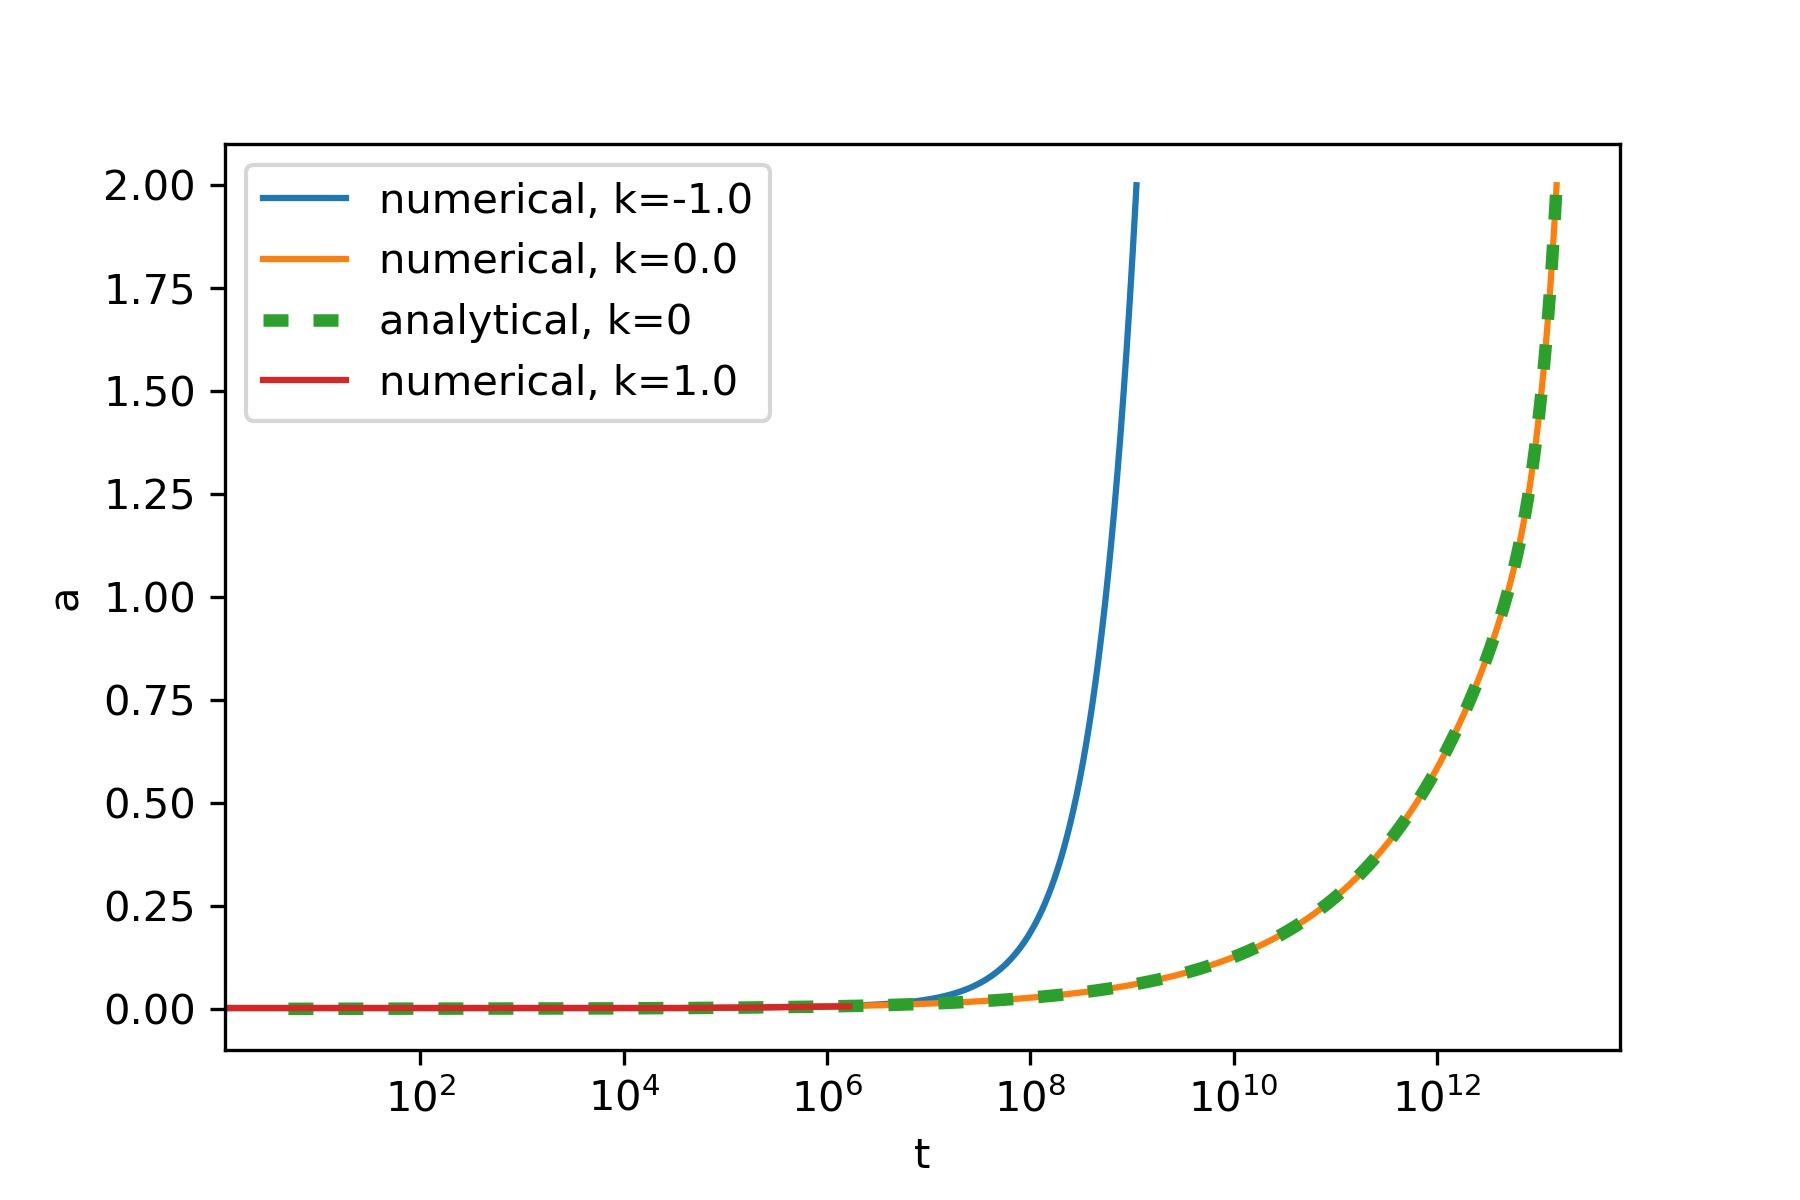
\includegraphics[scale=1]{Figures/a_ch.jpg}
\caption{Here equation (\ref{eq:NumSolMCG}) has been integrated numerically for $a'=0$ to $a'=1$ in incremental steps using the Gauss quadrature method. For this we have set $\frac{8\pi G}{3c^{2}}=\frac{c^{2}}{\chi^{2}}=1$ in order to investigate the behaviour of the model without looking at the physical constraints, and taken all of the free parameters to be the same as in the previous case. }
\label{fig:ChScale}
\end{figure}
In figure \ref{fig:ChScale} it can be seen that the numerically generated and analytical solution for the flat curvature case are in agreement. The scale factor increases slightly faster in later periods for an open curvature than for the flat case and slightly slower for the case of closed curvature.
\section{Behaviour of various quantities for the case of a Chaplygin equation of state}
In this section we aim to look at the behaviour of the Hubble parameter and acceleration for the case of a Chaplygin equation of state.
\subsection{The Hubble parameter for the case of a Chaplygin equation of state}
Taking the dimensionless Hubble parameter $h\equiv\frac{H}{H_{0}}$ and rewriting equation (\ref{eq:CurvFriedman}) we have that 
\begin{equation}\label{eq:HubbleParm}
\begin{split}
H &= \brac{A\rho -\kappa\frac{F}{a^{2}}}^{\frac{1}{2}},\\
\end{split}
\end{equation}
from which follows that 
\begin{equation}\label{eq:DimHubbleParm}
\begin{split}
h &= \frac{1}{H_{0}}\brac{A\rho -\kappa\frac{F}{a^{2}}}^{\frac{1}{2}}.\\
\end{split}
\end{equation}
Substituting equation (\ref{eq:ReFMCG}) into this gives
\begin{equation}\label{eq:ChDimHubbleParm}
\begin{split}
h &= \frac{1}{H_{0}}\bracc{A\brac{B_{3}a^{-3\brac{\beta}\brac{B_{1}}}+B_{2}}^{\frac{1}{\beta}} -\kappa\frac{F}{a^{2}}}^{\frac{1}{2}}.\\
\end{split}
\end{equation}
We can also let $a=\frac{1}{1+z}$, where $z$ is the red-shift and substitute this into equation (\ref{eq:ChDimHubbleParm}):
\begin{equation}\label{eq:zChDimHubbleParm}
\begin{split}
h(z) &= \frac{1}{H_{0}}\bracc{A\brac{B_{3}\brac{1+z}^{3\brac{\beta}\brac{B_{1}}}+B_{2}}^{\frac{1}{\beta}} -\kappa F\brac{1+z}^{2}}^{\frac{1}{2}}.\\
\end{split}
\end{equation}
This is done as the dimensionless Hubble parameter and red-shift can better be correlated to observational expectations. The behaviour of the dimensionless Hubble parameter can be seen in figure \ref{fig:ChH}.
\begin{figure}[H]
\centering
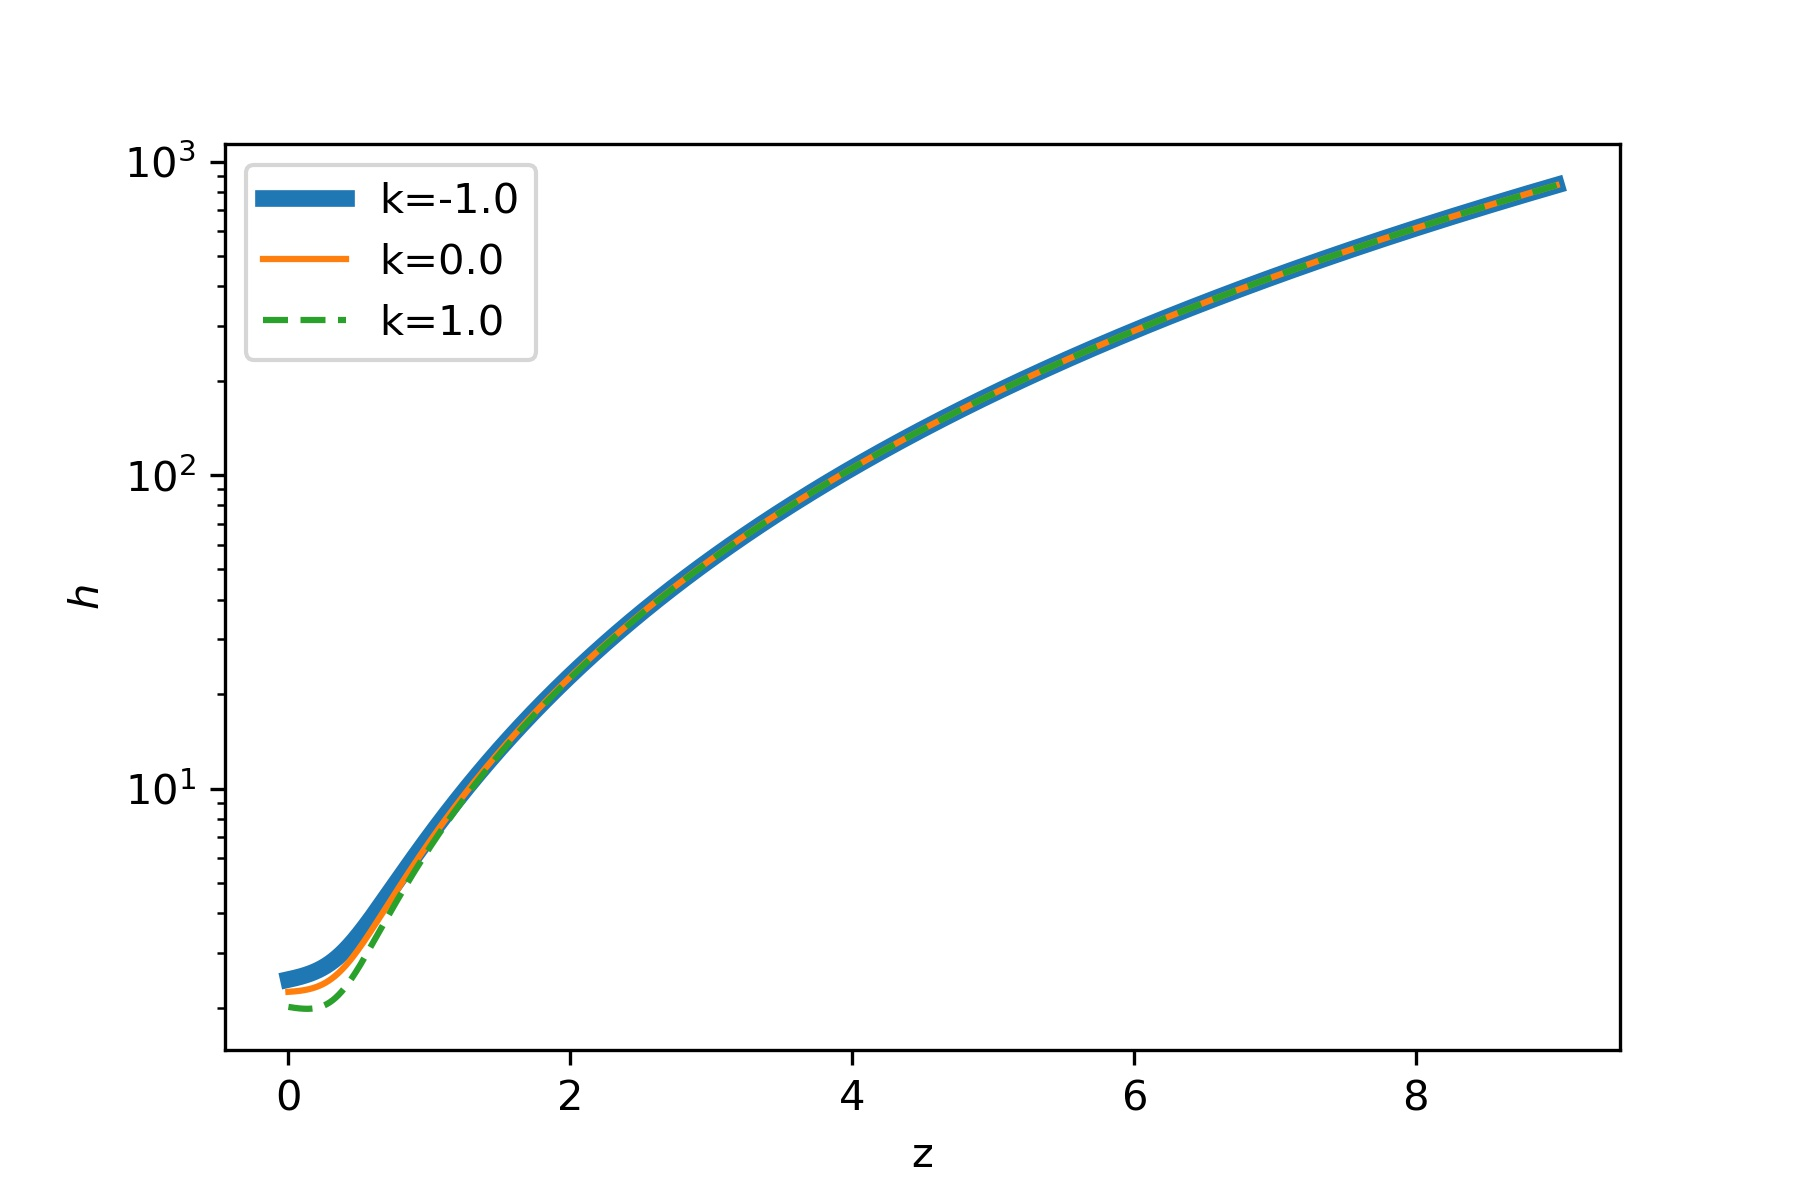
\includegraphics[scale=0.9]{Figures/ch_H.jpg}
\caption{Here the parameters have, again, been taken as in the previous cases and we have also set $H_{0}=1$.}
\label{fig:ChH}
\end{figure}

Rewriting equation (\ref{eq:zChDimHubbleParm}) we can define two new observable parameters, the fractional energy density parameter ($\Omega$):
\begin{equation}\label{eq:ChFracEnDen}
\begin{split}
h(z)^{2} &= \frac{A}{H_{0}^{2}}\brac{B_{3}\brac{1+z}^{3\brac{\beta}\brac{B_{1}}}+B_{2}}^{\frac{1}{\beta}} -\frac{\kappa F}{H_{0}^{2}}\brac{1+z}^{2}\\
&= \Omega_{Chap}(z)+\Omega_{\kappa}(z),\\
\end{split}
\end{equation}
where $\Omega_{chap}(z)$ is the fractional energy density of the Chaplygin gas fluid and $\Omega_{\kappa}(z)$ is the fractional energy density of the curvature of the universe.
\begin{figure}[H]
\centering
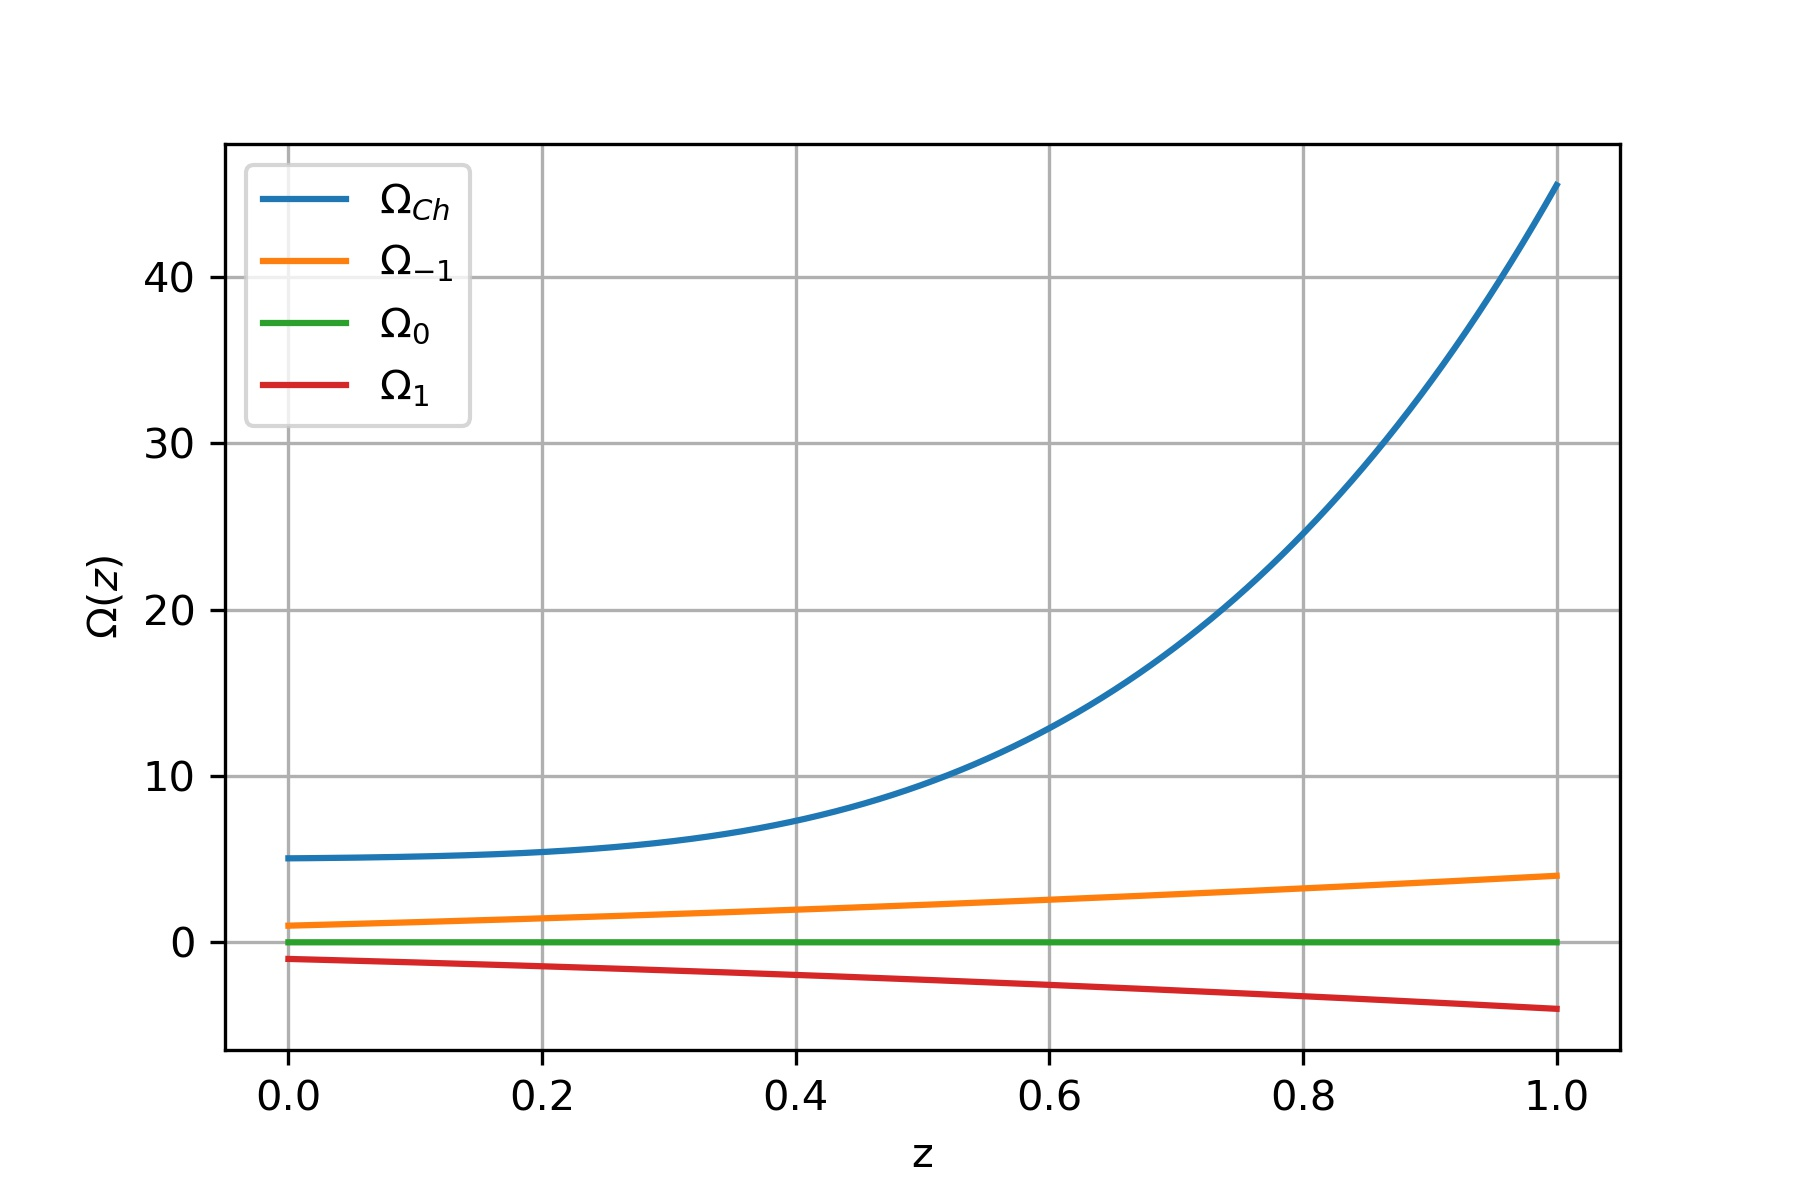
\includegraphics[scale=0.9]{Figures/ch_Om.jpg}
\caption{Taking the various parameters as in the previous cases, the figure shows the fractional energy density of the Chaplygin gas fluid as well as for the different curvature cases.It is important to point out here that the fractional energy density of the different curvatures are non-linear, but increases much slower than the Chaplygin gas fractional energy density for the chosen parameters.}
\label{fig:ChFracEnDen}
\end{figure}
In figure \ref{fig:ChFracEnDen} we see that the magnitudes of the fractional energy densities for both curvature and Chaplygin gas are of the order of unity for small red-shifts, as is expected. It is also evident that the fractional energy density of the Chaplygin gas increases much faster than that of the curvature term.
\subsection{Acceleration of the expansion for the case of a Chaplygin gas equation of state}
Substituting the equation of state (\ref{eq:MCG}) and energy density solution (\ref{eq:FMCG}) for the Chaplygin gas into the Raychaudhuri equation (\ref{eq:RayEq}) gives:
\begin{equation}\label{eq:ChRaych}
\begin{split}
\frac{\ddot{a}}{a} &= -\frac{A}{2}\brac{\brac{3B_{1}-2}\brac{B_{3}a^{-3B_{1}\beta}+B_{2}}^{\frac{1}{\beta}}-3B_{1}B_{2}\brac{B_{3}a^{-3\beta B_{1}}+B_{2}}^{\frac{1-\beta}{\beta}}},\\
\end{split}
\end{equation}
which is the normalized acceleration of the scale factor. The behaviour of the normalized acceleration can be seen in figure \ref{fig:ChAcc} and is initially decelerating as a high order polynomial but reduces to a constant acceleration close to a scale factor value of $a=1$, which corresponds to expectations from observation as well as what is expected for the Chaplygin gas equation of state.

\begin{figure}[H]
\centering
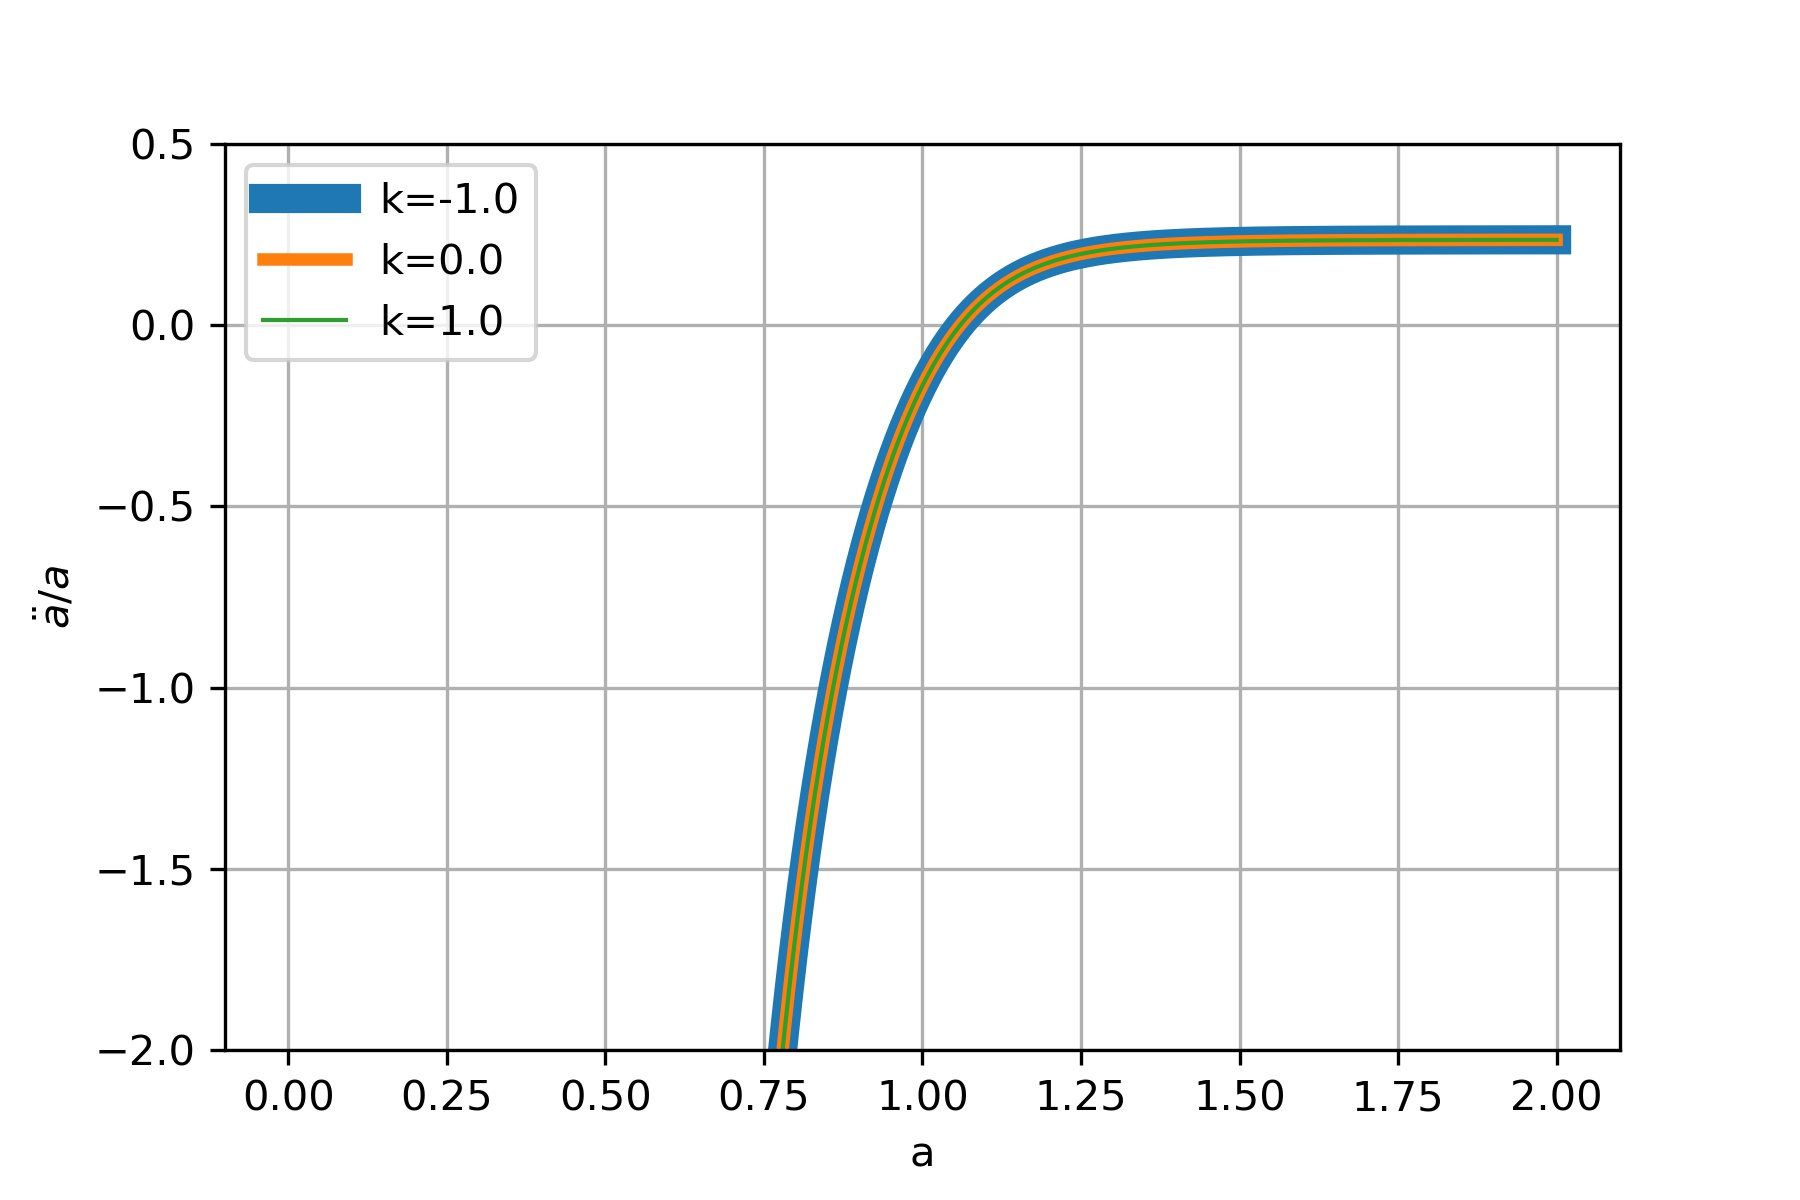
\includegraphics[scale=0.9]{Figures/ch_ddota.jpg}
\caption{Here the free parameters have again been taken to be as in the previous cases, which corresponds to $B_{1}=2$, $B_{2}=25$ and $B_{3}=\frac{1}{2}$. All other constants have also been normalized as in the previous cases.}
\label{fig:ChAcc}
\end{figure}

From equation (\ref{eq:ChRaych}) and equation (\ref{eq:ChDimHubbleParm}), we can also find an equation for the deceleration parameter $q$, defined in equation (\ref{eq:Deceleration}). We can rewrite $q$ as:
\begin{equation}\label{eq:ChModDecel}
\begin{split}
q &= -\frac{\ddot{a}}{a}\brac{\frac{1}{H}}^{2}         \\
&= \frac{\frac{A}{2}\brac{\brac{3B_{1}-2}\brac{B_{3}a^{-3B_{1}\beta}+B_{2}}^{\frac{1}{\beta}}-3B_{1}B_{2}\brac{B_{3}a^{-3\beta B_{1}}+B_{2}}^{\frac{1-\beta}{\beta}}}}{A\brac{B_{3}a^{-3\brac{\beta}\brac{B_{1}}}+B_{2}}^{\frac{1}{\beta}} -\kappa\frac{F}{a^{2}}},
\end{split}
\end{equation}
and again substitute $a=\brac{1+z}^{-1}$, to find the deceleration parameter as a function of red-shift:
\begin{equation}\label{eq:ChModDecelZ}
\begin{split}
q &= \frac{\frac{A}{2}\brac{\brac{3B_{1}-2}\brac{B_{3}\brac{1+z}^{3B_{1}\beta}+B_{2}}^{\frac{1}{\beta}}-3B_{1}B_{2}\brac{B_{3}\brac{1+z}^{3\beta B_{1}}+B_{2}}^{\frac{1-\beta}{\beta}}}}{A\brac{B_{3}\brac{1+z}^{3\brac{\beta}\brac{B_{1}}}+B_{2}}^{\frac{1}{\beta}} -\kappa F\brac{1+z}^{2}}.
\end{split}
\end{equation}
The behaviour of equation (\ref{eq:ChModDecelZ}) for all three different curvatures can be seen in figure \ref{fig:ChDecel}. 
\begin{figure}[H]
\centering
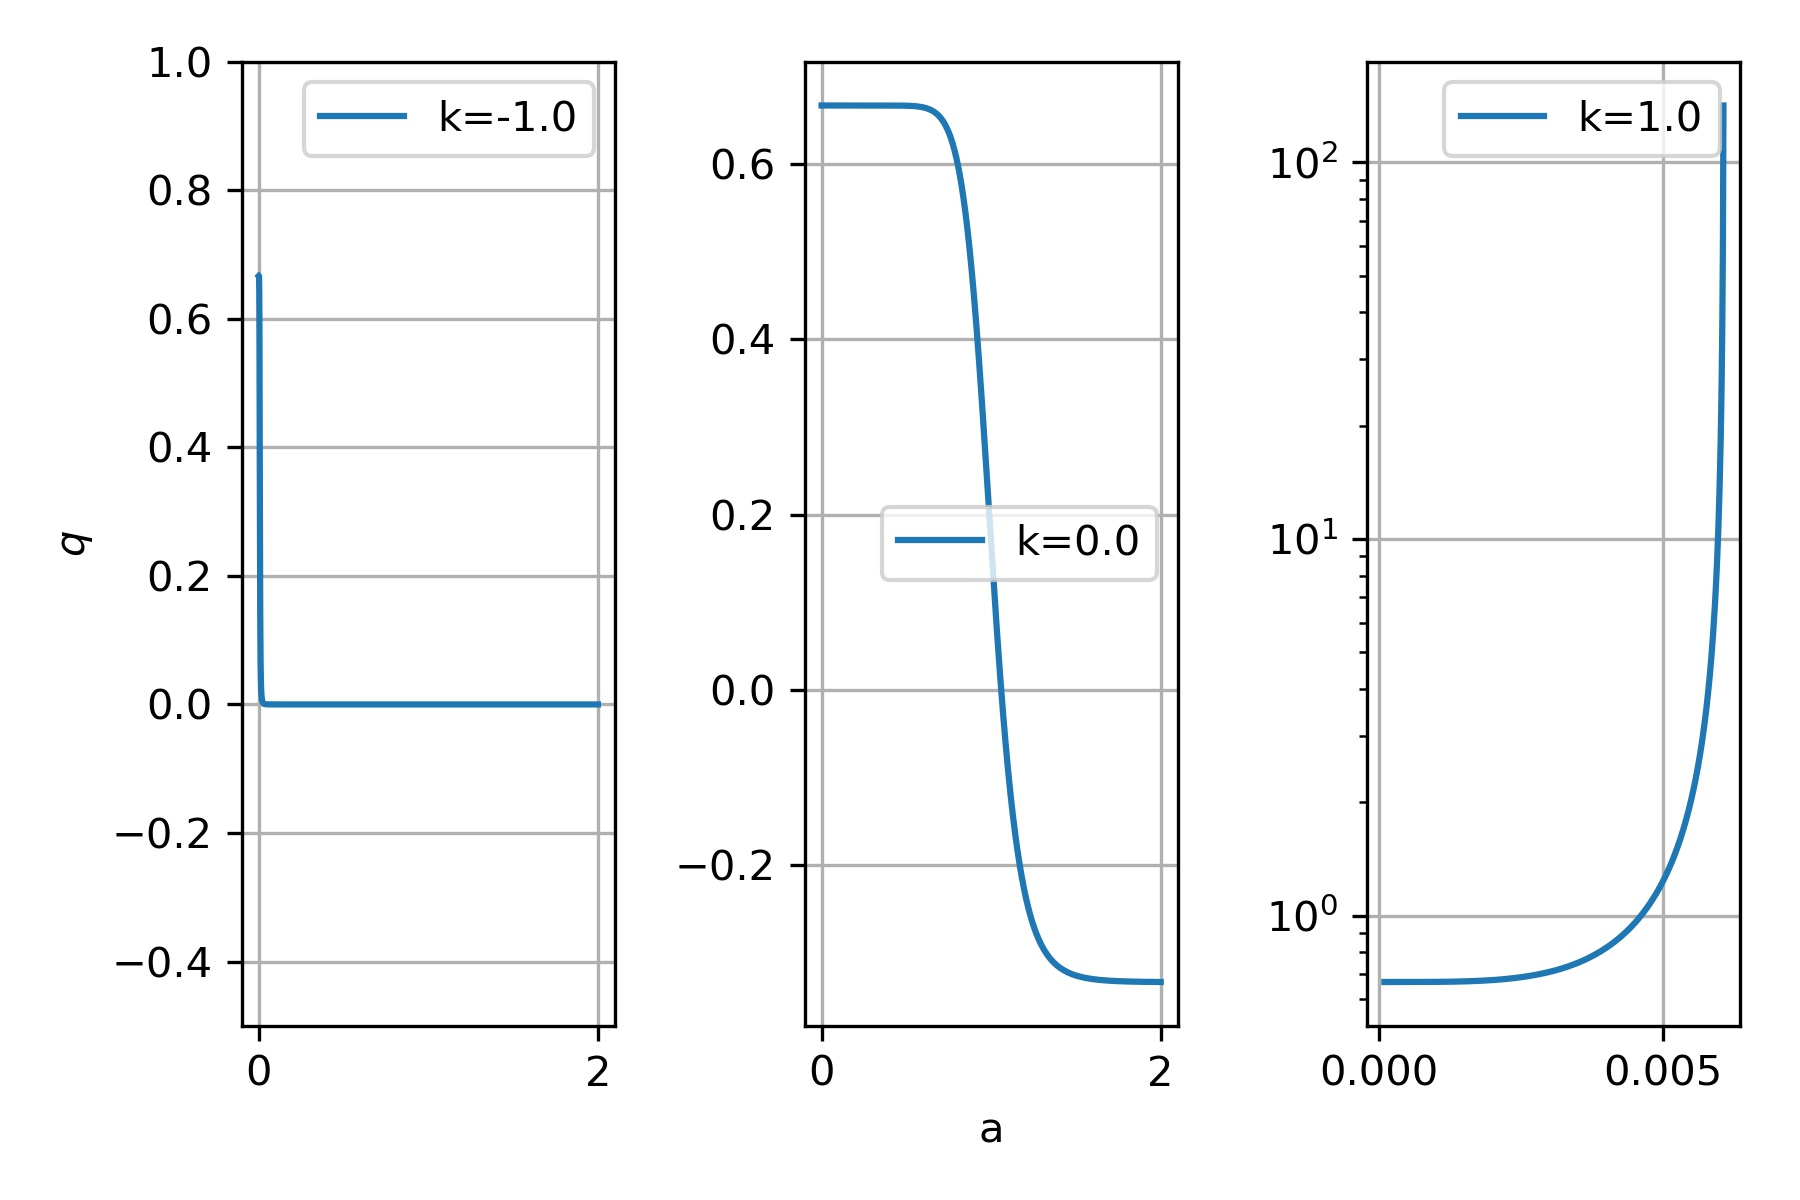
\includegraphics[scale=0.8]{Figures/ch_q.jpg}
\caption{Here all parameters and constants have again been normalized and taken as in the previous figures.}
\label{fig:ChDecel}
\end{figure}
From the figure it can be seen that for small red-shifts the deceleration parameter is negative which corresponds to an accelerated expansion. For large red-shifts, the deceleration parameter is positive corresponding to a decelerating universe. The figure also shows a relatively sharp change from positive to negative for the deceleration parameter.


\chapter{Unified dark Fluid}
Another possible candidate for dark energy that also aims to unify dark energy and dark matter into a single dark fluid is proposed by \textit{Wang, Yan and Meng} \citep{wang2017new}. The proposed candidate is a perfect fluid equation of state $P=\omega\rho$ that is parametrized between an equation of state that describes a matter (and here by dark matter) dominated universe, and a dark energy dominated universe. 
\section{The Pressure-Parametrized Unified dark Fluid equation of state}
The proposed equation of state is given as:
\begin{equation}\label{eq:UDFEoS}
\begin{split}
P &= P_{a}+P_{b}\brac{a^{-1}-a},         \\
\end{split}
\end{equation}
with $P_{a}$ and $P_{b}$ free parameters that are to be constrained by observation.
\paragraph{Solving the fluid equation for the proposed equation of state}
Substituting equation (\ref{eq:UDFEoS}) into the fluid equation (\ref{eq:4}), gives:
\begin{equation}\label{eq:UDFFluid}
\begin{split}
\dot{\rho} &= -3\brac{\frac{\dot{a}}{a}}\brac{\rho+P_{a}+P_{b}\brac{a^{-1}-a}}. \\
\end{split}
\end{equation}
Solving this first order differential equation we find the energy density to be:\begin{equation}\label{eq:UDFFluidSol}
\begin{split}
\rho&= -P_{a}+\frac{3}{4}P_{b}\brac{a-2a^{-1}}+Ca^{-3}, \\
\end{split}
\end{equation}
where $C$ is an integration constant. Comparing the found solution to the energy densities found for the Concordance model, it can be seen that the first term in equation (\ref{eq:UDFFluidSol}) corresponds to that of a dark energy dominated epoch, while the last term corresponds to that of a dust dominated epoch.
Again converting equation (\ref{eq:UDFFluidSol}) from scale factor to red-shift:
\begin{equation}\label{eq:UDFFluidSolZ}
\begin{split}
\rho&= -P_{a}+\frac{3}{4}P_{b}\bracc{\brac{1+z}^{-1}-2\brac{1+z}}+C\brac{1+z}^{3}, \\
\end{split}
\end{equation}
and plotting the result, we can see the behaviour of the energy density for the pressure-parametrized unified dark fluid (PPUDF) equation of state.

\begin{figure}[H]
\centering
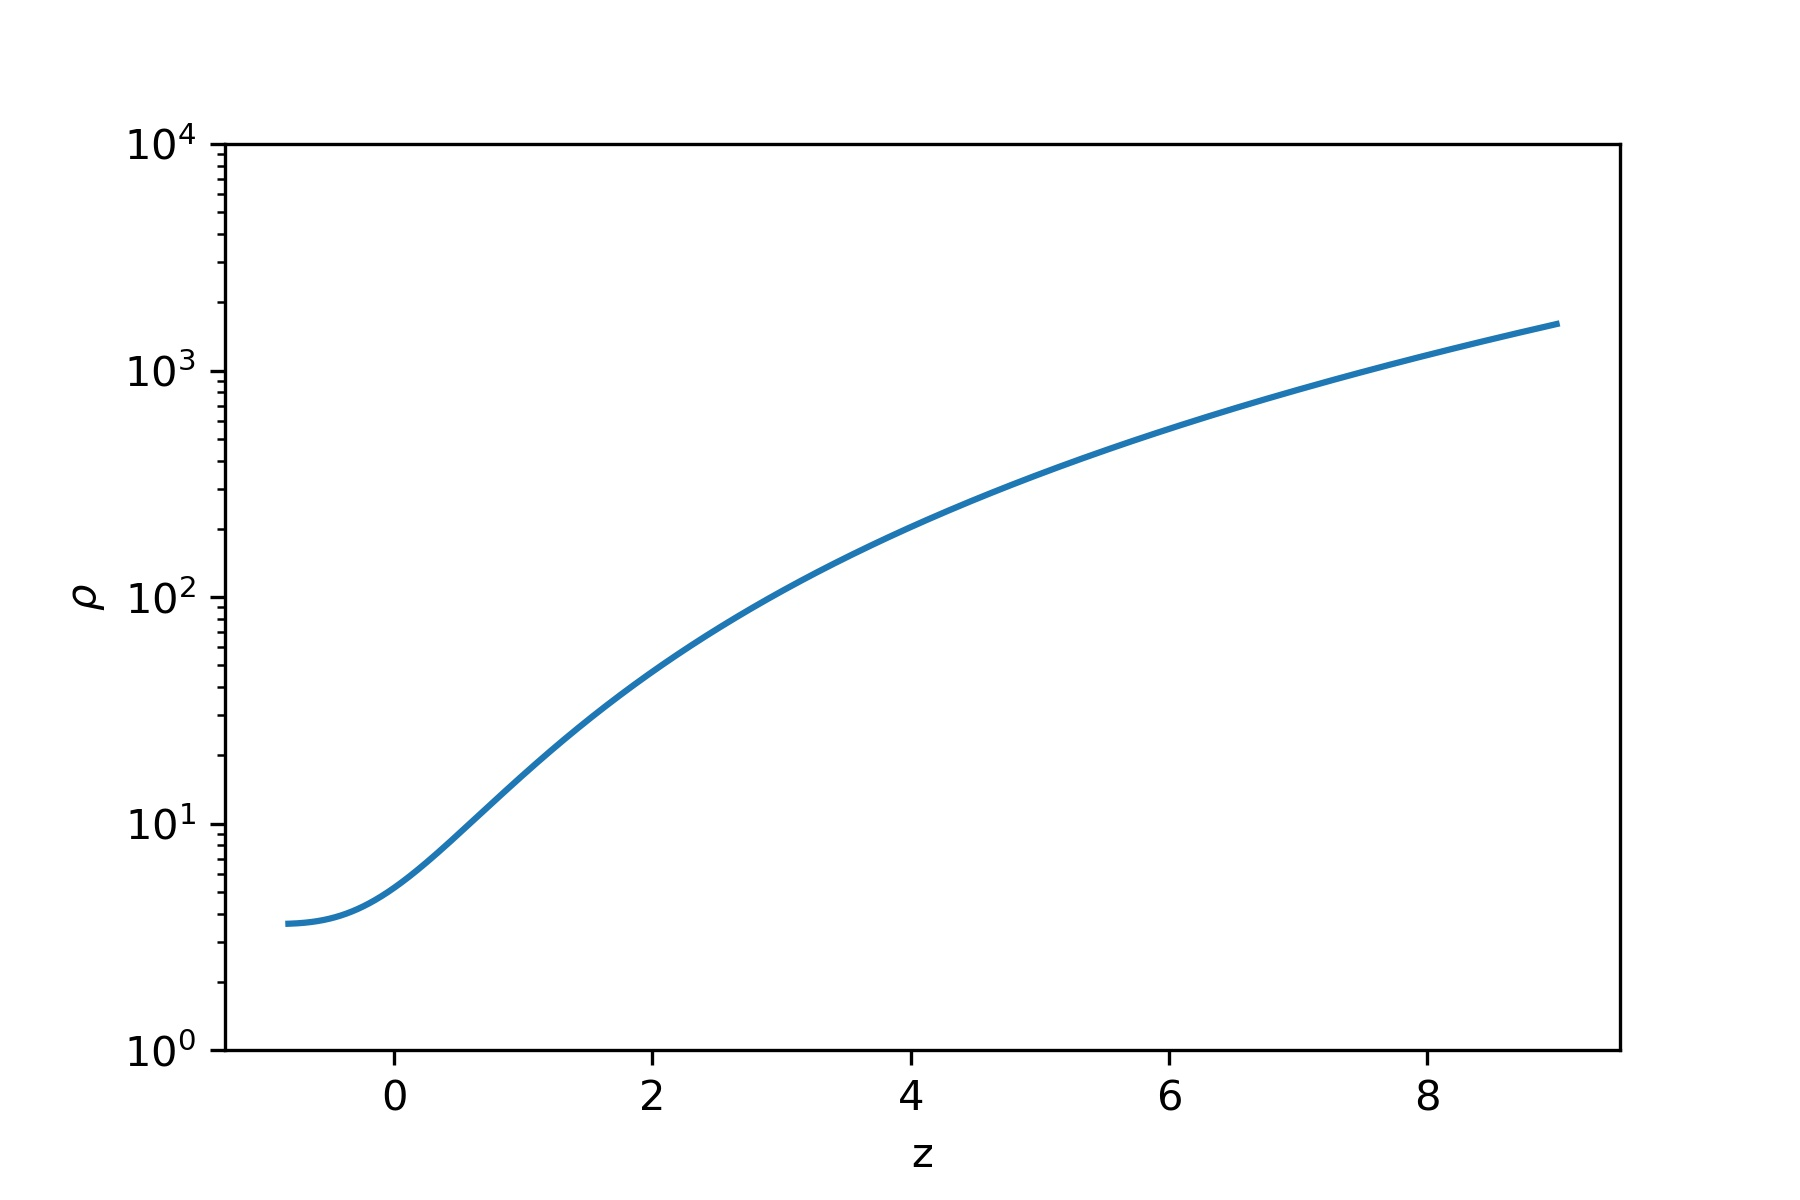
\includegraphics[scale=1]{Figures/UDF_rho.jpg}
\caption{Here we have arbitrarily taken $P_{a}=-3.6$, $P_{b}=-10^{-5}$ and $C=1.6$.}
\label{fig:UDFRho}
\end{figure}
In figure \ref{fig:UDFRho} it can be seen that the energy density increases non-linearly with red-shift, as is expected. It is worth pointing out here that the energy density is sensitive to the values of the free parameters. The plot has also been extended into negative red-shifts to show that the energy density does reduce to an approximately constant energy density in the near future.

\section{Behaviour of various quantities for the case of the PPUDF equation of state}
In this section we again aim to look at the behaviour of the dimensionless Hubble parameter, acceleration and other associated values for the case of a PPUDF equation of state.
\subsection{The Dimensionless Hubble parameter for the case of a PPUDF equation of state}
Using the same definition as before, we can find an expression for the dimensionless Hubble parameter as a function of red-shift. Substituting equation (\ref{eq:UDFFluidSolZ}) into equation (\ref{eq:DimHubbleParm}), we have:
\begin{equation}\label{eq:UDFDimh}
\begin{split}
h &= \frac{1}{H_{0}}\bracc{A\brac{-P_{a}+\frac{3}{4}P_{b}\bracc{\brac{1+z}^{-1}-2\brac{1+z}}+C\brac{1+z}^{3}} -\kappa F \brac{1+z}^{2}}^{\frac{1}{2}}.\\
\end{split}
\end{equation}
As can be seen in figure \ref{fig:UDFh}, for the case of a PPUDF equation of state, the dimensionless Hubble parameter increases non-linearly with red-shift. Further more the $h$ is of the order of unity for small red-shifts, as is expected from observation. 

\begin{figure}[H]
\centering
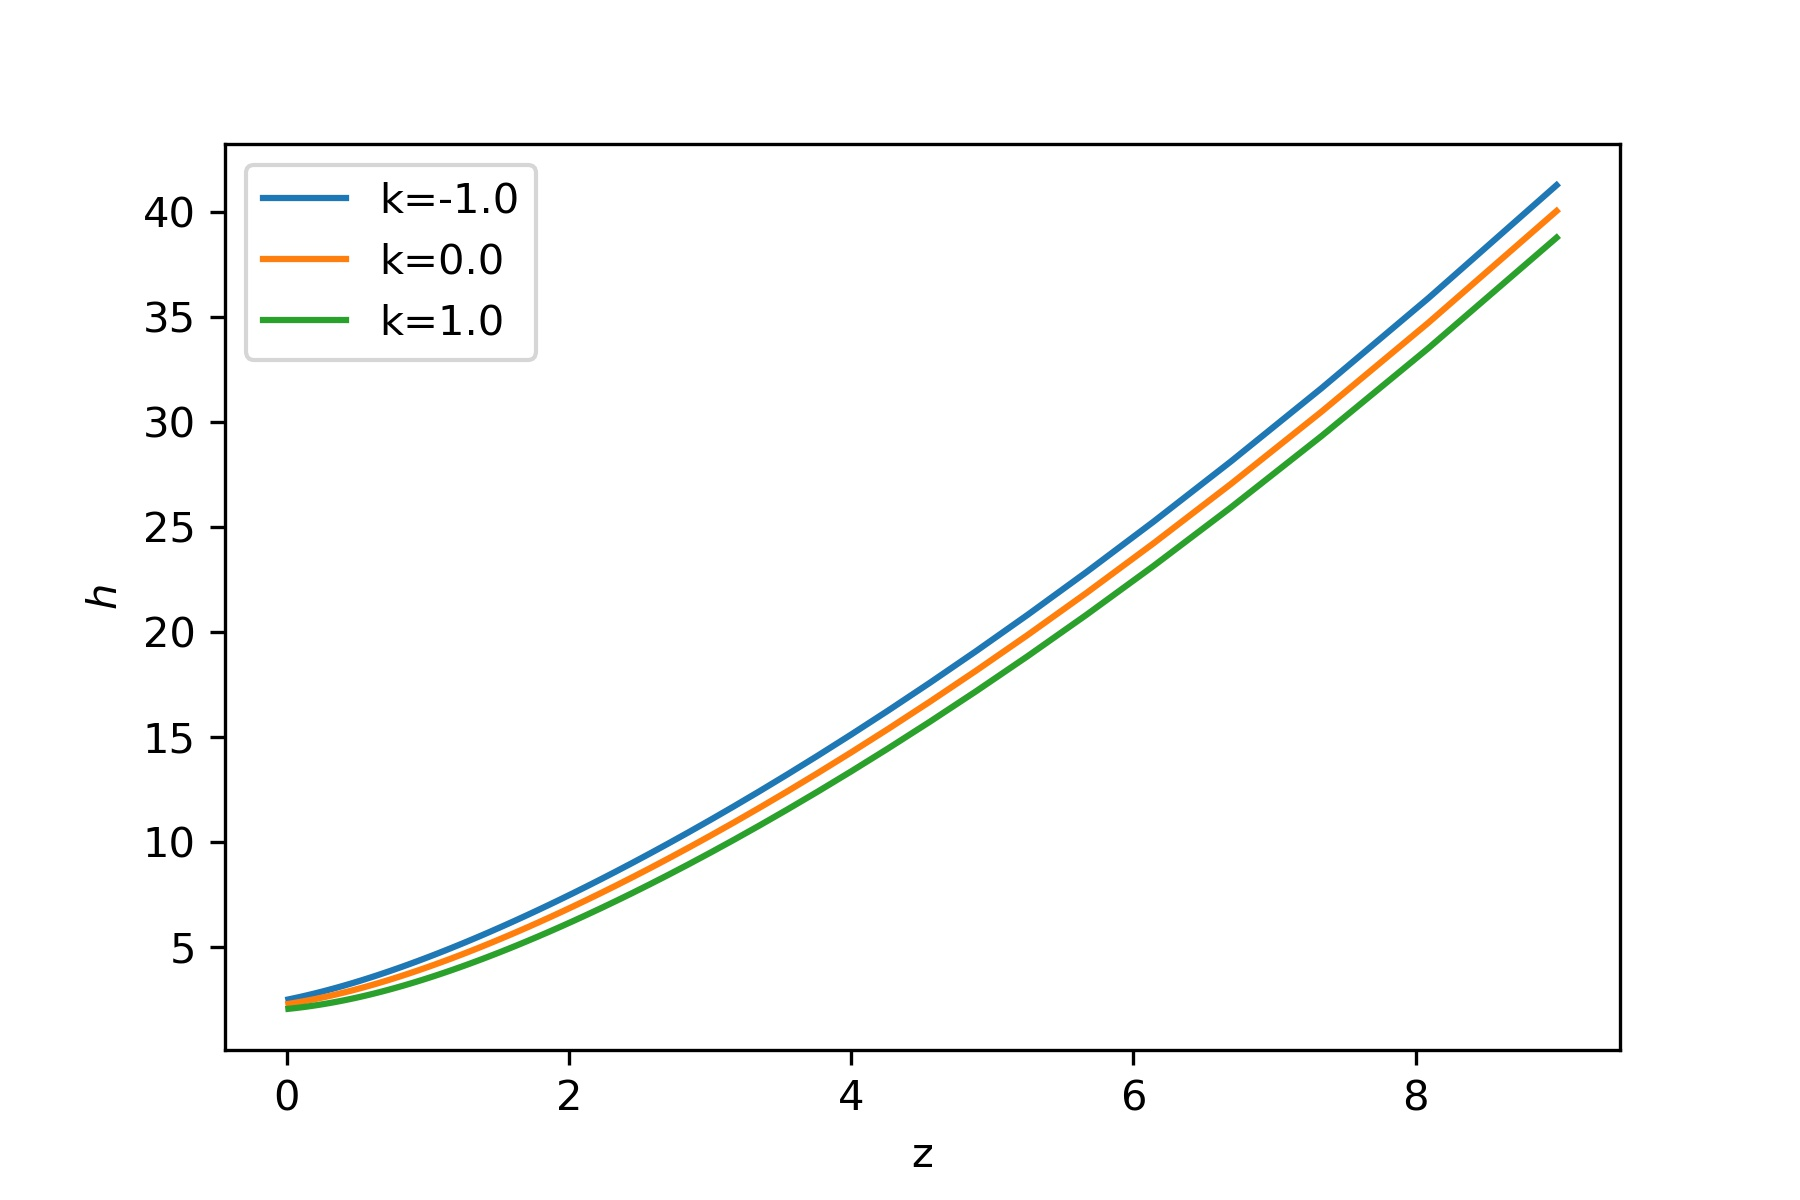
\includegraphics[scale=1]{Figures/UDF_H.jpg}
\caption{Here we have again taken $H_{0}=A=F=1$ and taken the free parameters as before.}
\label{fig:UDFh}
\end{figure}

Defining the fractional energy density for the PPUDF case $\Omega_{PPUDF}$ as:
\begin{equation}\label{eq:UDFOmega}
\begin{split}
\Omega_{PPUDF}(z) &\equiv \frac{A}{H_{0}^{2}}\brac{-P_{a}+\frac{3}{4}P_{b}\bracc{\brac{1+z}^{-1}-2\brac{1+z}}+C\brac{1+z}^{3}},       \\
\end{split}
\end{equation}
and keeping the fractional energy density of curvature as before, we can look at the behaviour of the fractional energy densities for the case of a PPUDF equation of state.
\begin{figure}[H]
\centering
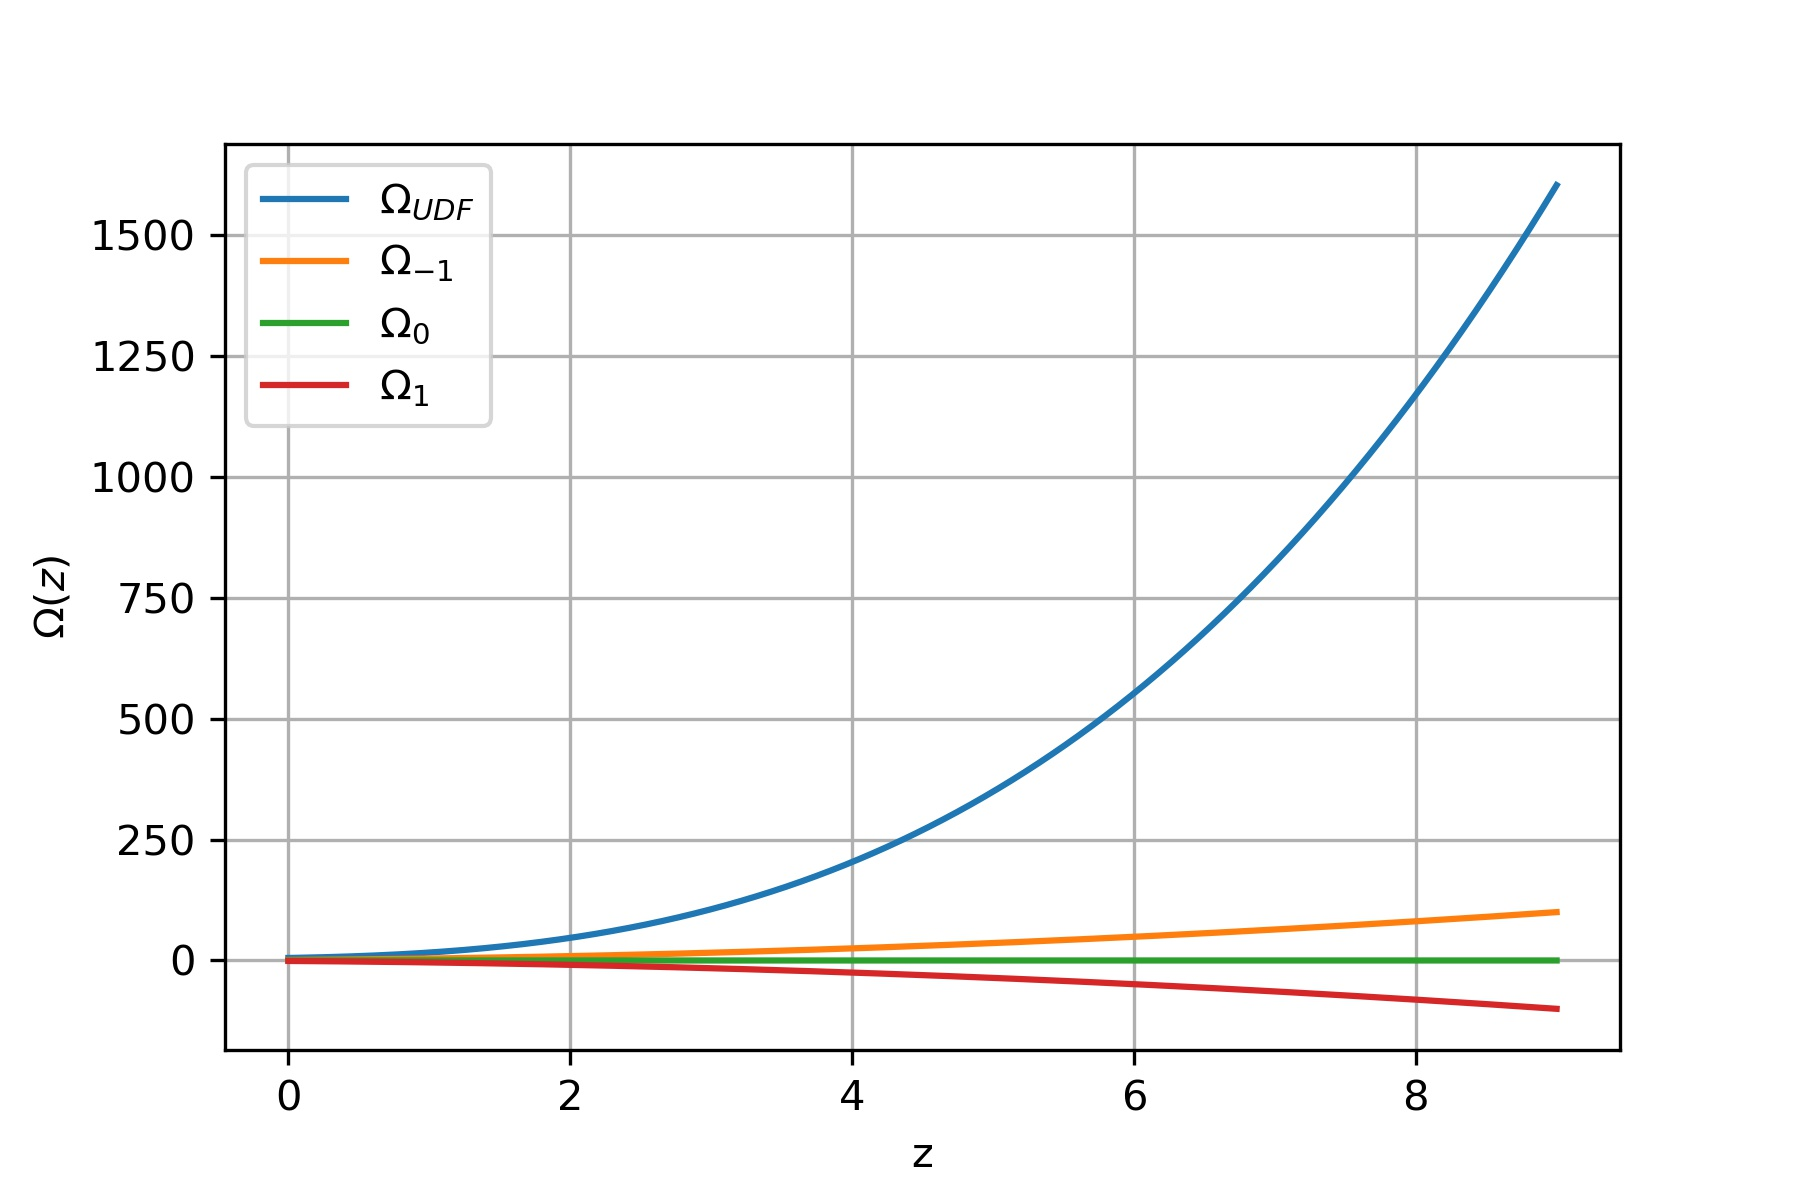
\includegraphics[scale=1]{Figures/UDF_Om.jpg}
\caption{All constants and parameters have been taken as in the previous figures. It is again important to point out that, as in the previous case, the fractional energy density of the different curvatures are non-linear, but increases much slower than the PPUDF fractional energy density for the chosen parameters.}
\label{fig:UDFOmega}
\end{figure}
From figure \ref{fig:UDFOmega} it is clear that the fractional energy density for the PPUDF increases much faster than that of curvature with red-shift, but is comparable to that of curvature for small red-shifts. 


\subsection{Acceleration of the scale factor for the case of the PPUDF equation of state}
Substituting the equation of state (\ref{eq:UDFEoS}) and resulting energy density (\ref{eq:UDFFluidSol}) for the PPUDF into the Raychaudhuri equation (\ref{eq:RayEq}), we have:
\begin{equation}\label{eq:RayUDF}
\begin{split}
\frac{\ddot{a}}{a} &= -\frac{A}{2}\bracc{2P_{a}-\frac{3}{2}P_{b}\brac{\frac{3}{2}a+a^{-1}}+Ca^{-3}}.\\
\end{split}
\end{equation}
From this it is clear that for large values of the scale factor, the Raychaudhuri equation becomes approximately linear. This corresponds with observation, and also suggests that the parameter $P_{b}$ must be small to correspond with an approximately constant acceleration as observational data suggests \citep{wang2017new}. From figure \ref{fig:UDFRay} it is clear that the PPUDF equation of state supports an expansion that is initially decelerating, but changes to an accelerating expansion with a close to constant acceleration.

\begin{figure}[H]
\centering
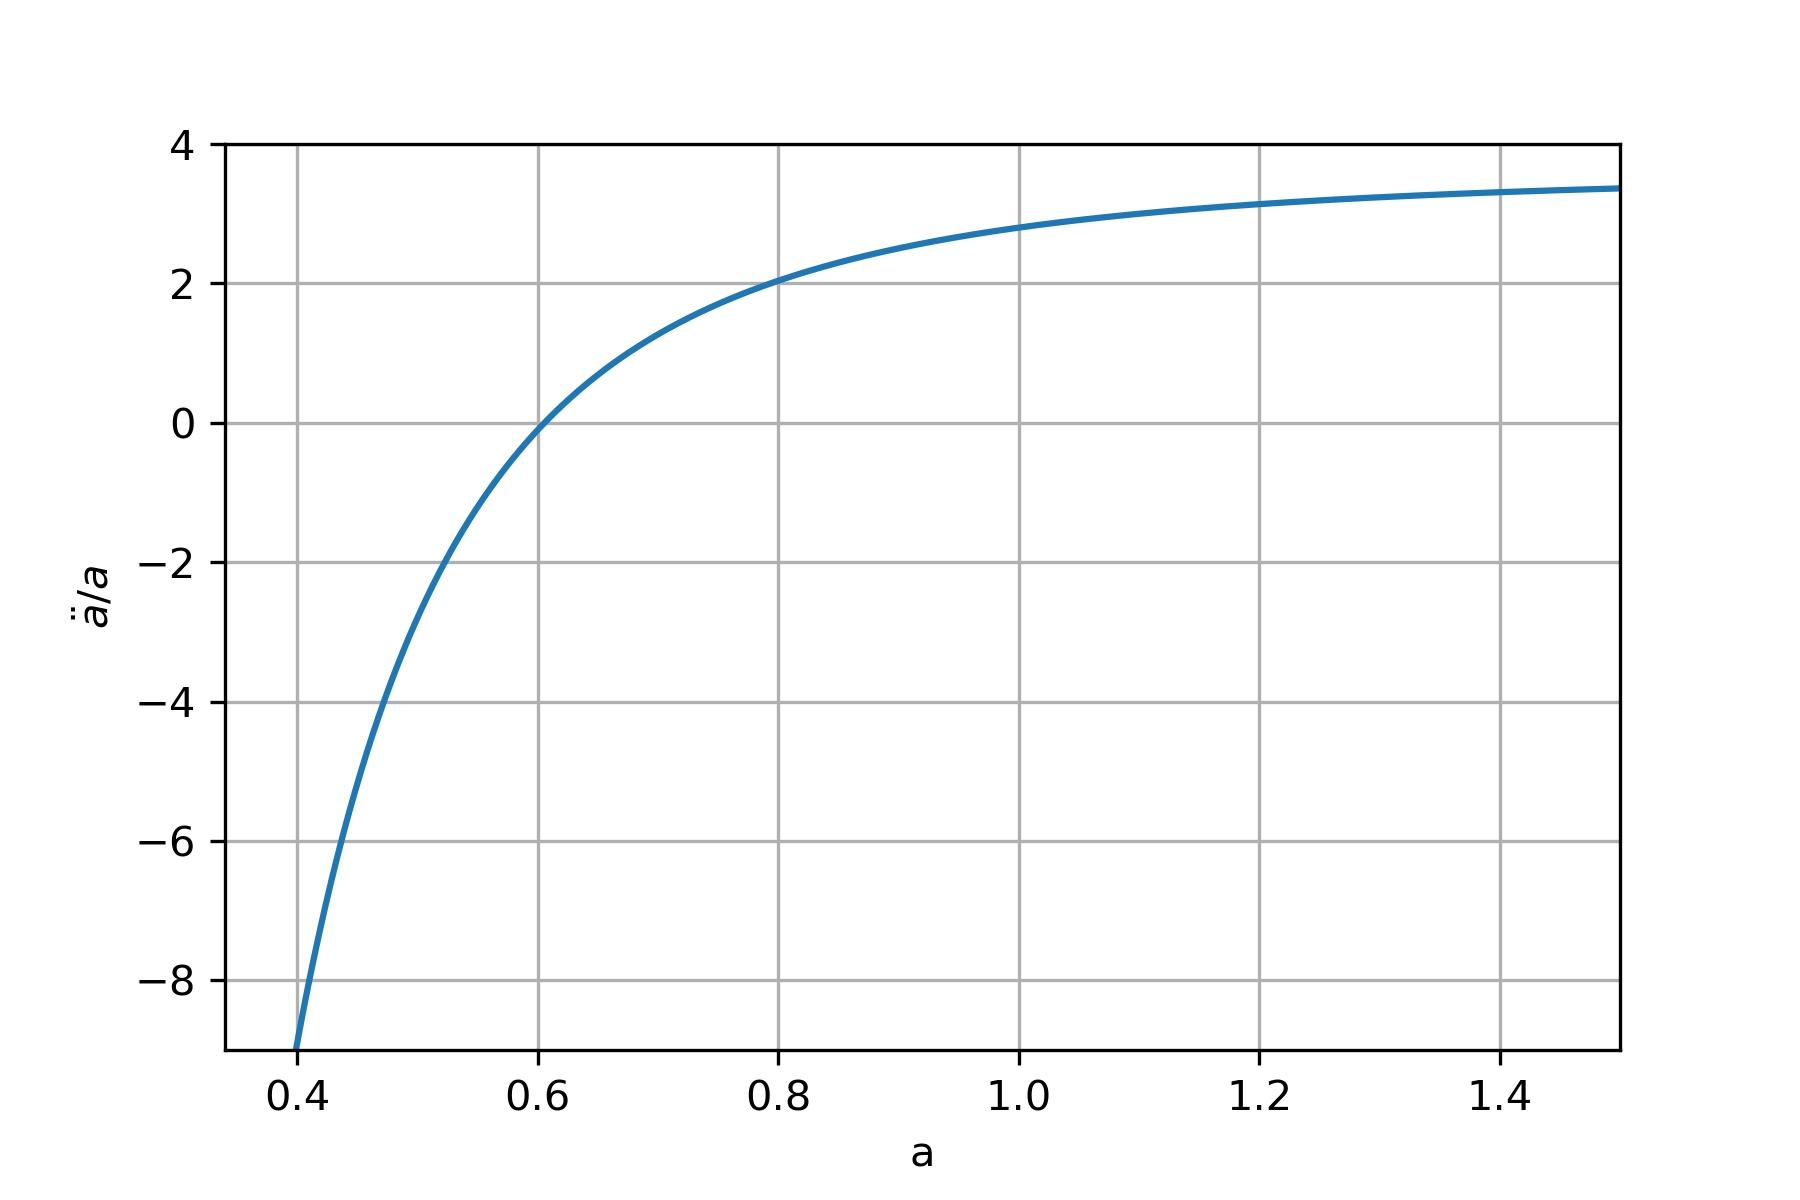
\includegraphics[scale=1]{Figures/UDF_addot.jpg}
\caption{All parameters and constants have again been taken as for the previous figures. The plot has been extended to a scale factor of $a=1.5$ to illustrate that the acceleration becomes approximately linear and asymptotically constant.  }
\label{fig:UDFRay}
\end{figure} 
Taking the same approach to find an expression for the deceleration parameter as in equation (\ref{eq:ChModDecel}), we find that the deceleration parameter $q$ for the case of the PPUDF is:
\begin{equation}\label{eq:UDFq}
\begin{split}
q &= \frac{A\bracc{2P_{a}-\frac{3}{2}P_{b}\brac{\frac{3}{2}\brac{1+z}^{-1}+\brac{1+z}}+C\brac{1+z}^{3}}}{2A\brac{-P_{a}+\frac{3}{4}P_{b}\bracc{\brac{1+z}^{-1}-2\brac{1+z}}+C\brac{1+z}^{3}} -\kappa F \brac{1+z}^{2}}.        \\
\end{split}
\end{equation}
It is clear that the deceleration parameter is very sensitive to the values of the free parameters. In figure \ref{fig:UDFq} we again plot the resulting expression for the deceleration parameter as a function of red-shift in order to see the behaviour of the deceleration parameter.

\begin{figure}[H]
\centering
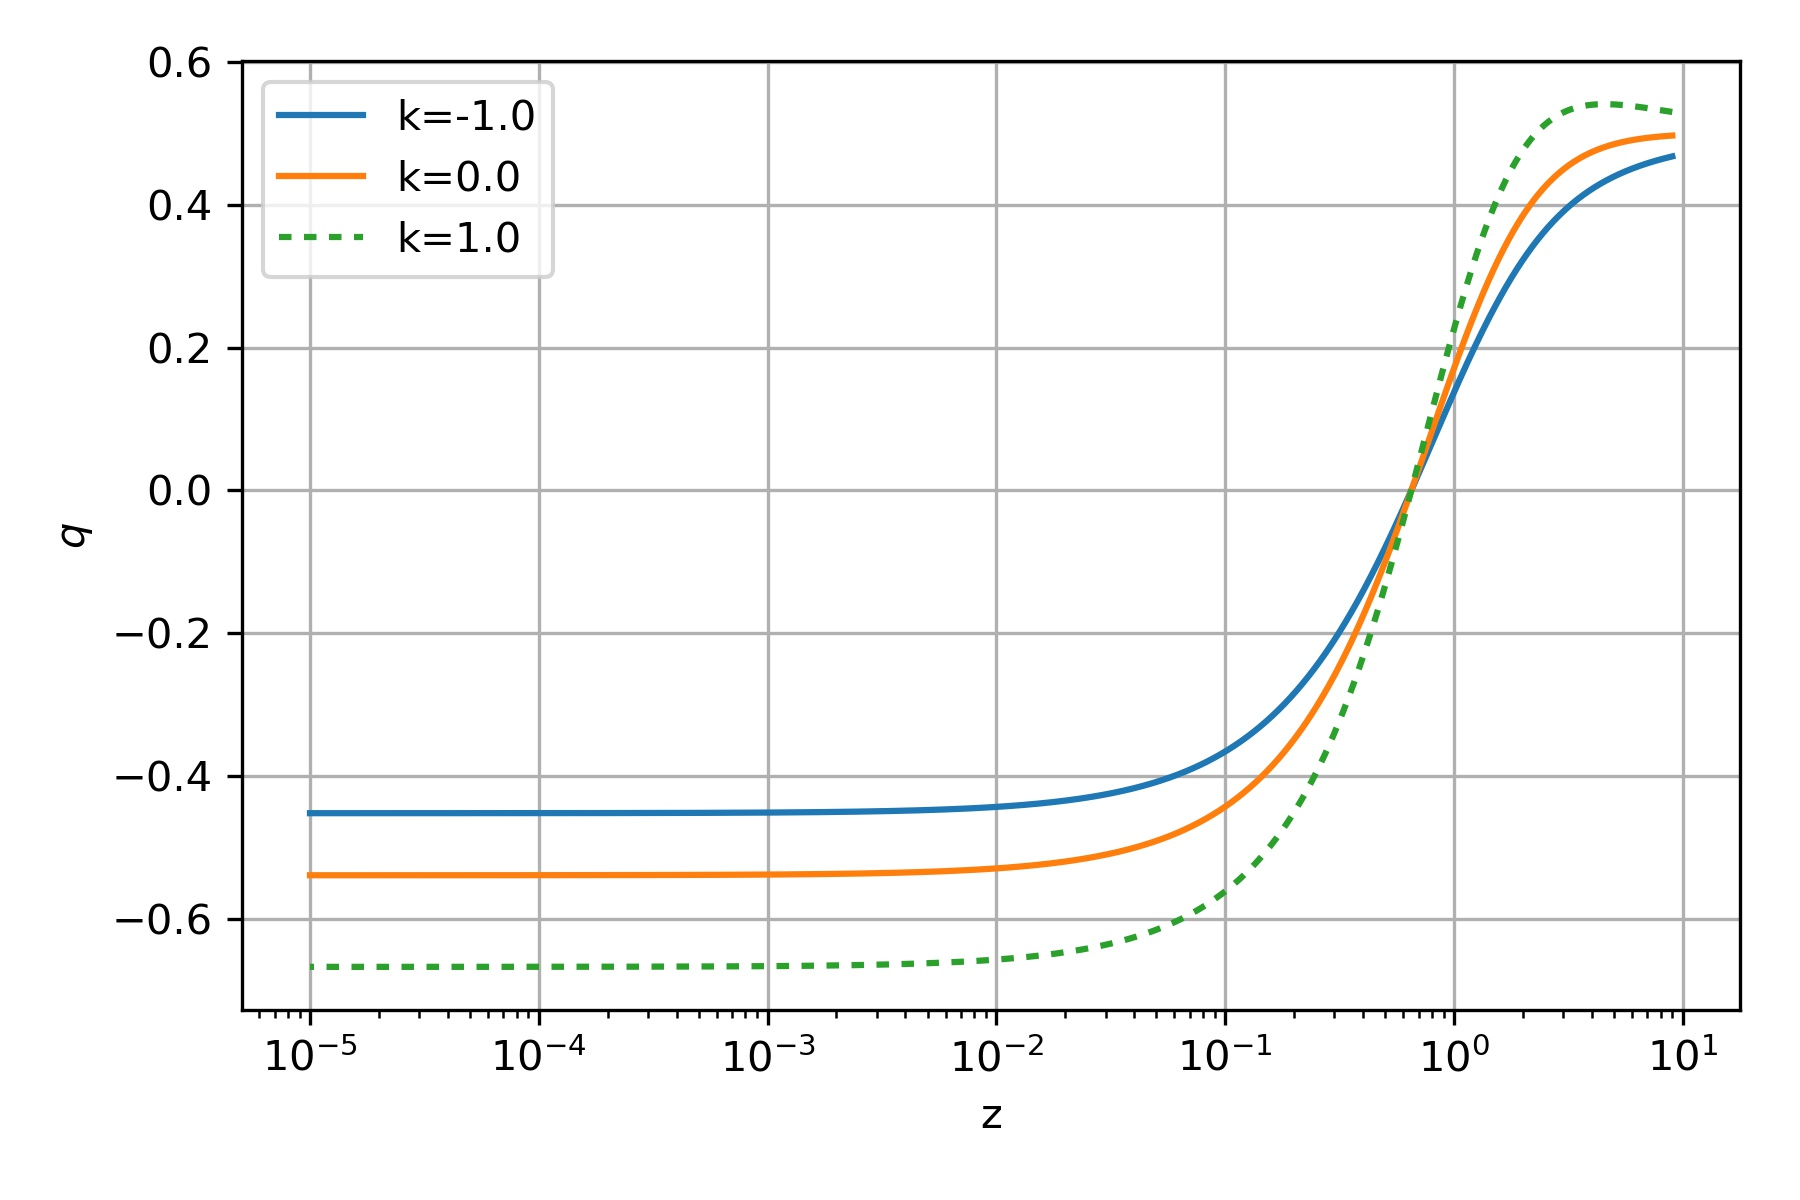
\includegraphics[scale=1]{Figures/UDF_q.jpg}
\caption{Here the free parameters and constants have been taken to be the same as for the previous figures.}
\label{fig:UDFq}
\end{figure}
It is clear from the figure that the PPUDF equation of state also supports a universe that is initially undergoing an approximately constant deceleration that rapidly changes to an approximately constantly accelerating universe for small reed-shifts.

\chapter{Final remarks}
\section{Discussion and Conclusions}
From figures \ref{fig:ChRho} and \ref{fig:UDFRho} it is clear that both the Chaplygin gas and the PPUDF equations of state show behaviour of the energy density that corresponds with that of the concordance model for both the dust and dark energy dominated epochs. Both equations of state result in an expression for energy density that is non-linear for large red-shifts. The expression for energy density that results from the Chaplygin gas equation of state also reduces to a constant for small red-shift. For the energy density expression that results from the PPUDF equation of state, figure \ref{fig:UDFRho} shows that the energy density deviates from the Concordance model for small red-shifts, but reduces to the concordance model in the near future which is consistent with the findings of \textit{Wang, Yan} and \textit{Meng} \citep{wang2017new}. Looking at the behaviour of the dimensionless Hubble parameter that results from using either equation of state, we find that both equations of state are viable when compared to what is expected based on observation. The behaviour of the deceleration parameter that results from both the PPUDF and Chaplygin gas equations of state, support an expansion that is initially decelerating, which then abruptly changes to a near constantly accelerating expansion. The former behaviour is consistent with a dust dominated epoch. The later is consistent with a dark energy dominated epoch. The behaviour resulting from both equations of state are very sensitive to the chosen values of the free parameters and must therefore be constrained by observation.\\
From the resulting behaviour found for both the PPUDF and Chaplygin gas equations of state, it is clear that it is possible to parametrize the equations of state for the dust dominated epoch and dark energy dominated epoch into that of a single unified dark fluid equation of state that is consistent with the Concordance model.

\section{Acknowledgements}
I wish to thank The National Astrophysics and Space Science (NASSP) and  Center for Space Research (CSR) for funding and support as well as Dr. Amare Abebe  and Dr. Bishop Mongwane for their support with the project.


\newpage
\chapter{Appendices}
\section*{Appendix A}
\subsection*{equation of State from Newtonian Mechanics}

\begin{equation}
\begin{split}
E(t) &= -PV(t)\\
\Rightarrow \dot{E} &= \frac{d\left(-PV\right)}{dt}\\
&= -\driv{P}{t}V-P\driv{V}{t}\\
&= -P\driv{V}{t}             \\
\end{split}
\end{equation}
since $P$ is a constant.
We have that for M the total mass and c the speed of light 
\begin{equation}
\begin{split}
V &= \frac{4\pi}{3}r^{3}\\
E &= Mc^{2}\\
&=\frac{4\pi}{3}c^{2}r^{3}\rho\\
\end{split}
\end{equation}
where $\rho$ is the mass density as a function of time.

Substituting equations (\ref{eq:Stuff1}) and (\ref{eq:Stuff2}) back into equation 3 yields
\begin{equation}
\begin{split}
\frac{4\pi\chi^{3} c^{2}}{3}\left(3a^{2}\dot{a}\rho+\dot{\rho}a^{3}\right) &= -P4\pi\chi^{3}a^{2}\dot{a}\\
\Rightarrow \dot{\rho}+3\frac{\dot{a}}{a}\rho+3P\frac{\dot{a}}{a} &= 0\\
\Rightarrow \dot{\rho}+3\frac{\dot{a}}{a}\left(\rho+P\right) &= 0\\
\Rightarrow \dot{\rho}+3H\left(\rho+P\right) &= 0\\
\end{split}
\end{equation}


Solving equation (\ref{eq:6}) 
\begin{equation}
\begin{split}
\dot{\rho}+3H\left(1+\omega\right)\rho &= 0\\
\Rightarrow \frac{\dot{\rho}}{\rho} &= -3H\left(1+\omega\right)\\
\Rightarrow \frac{\dot{\rho}}{\rho} &= -3\left(1+\omega\right)\frac{\dot{a}}{a}\\
\Rightarrow ln(\rho) &= -3\left(1+\omega\right)ln(a) + k\\
\Rightarrow \rho &= Ca^{-3\left(1+\omega\right)}
\end{split}
\end{equation}
with $C$ and $k$ constants.


\subsection*{The Expansion equation}

\begin{equation}
\begin{split}
m\ddot{R} &= -\frac{GMm}{R^{2}}\\
\end{split}
\end{equation}
Multiplying both sides of the equation with $\dot{R}$, dividing by $m$ and integrating over time gives
\begin{equation}
\begin{split}
\ddot{R}\dot{R} &= -\frac{GM}{R^{2}}\dot{R}\\
\Rightarrow\frac{1}{2}\dot{R}^2 &= \frac{GM}{R}+U\\
\end{split}
\end{equation}
Where $U$ is an integration constant. Since we have that $M=\frac{4\pi}{3}R^{3}\rho$ and $R=ar$, it follows that
\begin{equation}
\begin{split}
\frac{1}{2}\dot{R}^2 &= \frac{GM}{R}+U\\
\Rightarrow\frac{1}{2}\dot{a}^{2}r^{2} &= \frac{\frac{4\pi}{3}a^{3}r^{3}\rho G}{ar}+U\\
\Rightarrow\left(\frac{\dot{a}}{a}\right)^{2} &= \frac{8\pi}{3}G\rho+\frac{2U}{a^{2}r^{2}}\\
\end{split}
\end{equation}
which is the expansion equation, with $\rho$ the mass-density.

\subsection*{The Raychaudhuri equation}

From the the Friedman equation (\ref{eq:5}) we have that
\begin{equation}
\begin{split}
\left(\frac{\dot{a}}{a}\right)^{2} &= \frac{8\pi}{3}G\rho+\frac{2U}{a^{2}r^{2}}\\
\Rightarrow \dot{a}^{2} &= \frac{8\pi}{3}G\rho a^{2}+\frac{2U}{r^{2}}\\
\Rightarrow \driv{}{t}\left(\dot{a}^{2}\right) &= \driv{}{t}\left(\frac{8\pi}{3}G\rho a^{2}+\frac{2U}{r^{2}}\right)\\
\Rightarrow 2\dot{a}\ddot{a} &= \frac{8\pi}{3}G\left(2\rho a\dot{a}+\dot{\rho}a^{2}\right)\\
\end{split}
\end{equation}
dividing this by $2a\dot{a}$ and substituting in the equation of State (with $H=\frac{\dot{a}}{a}$) gives
\begin{equation}
\begin{split}
\Rightarrow \frac{\ddot{a}}{a} &= \frac{4\pi}{3}G\left(2\rho +\dot{\rho}\frac{a}{\dot{a}}\right)\\
\Rightarrow \frac{\ddot{a}}{a} &= \frac{4\pi}{3}G\left(2\rho -3H\left(1+\omega\right)\rho\frac{a}{\dot{a}}\right)\\
\Rightarrow \frac{\ddot{a}}{a} &= \frac{4\pi}{3}G\left(2\rho -3\left(1+\omega\right)\rho\right)\\
\Rightarrow \frac{\ddot{a}}{a} &= -\frac{4\pi}{3}G\left(\rho +3\omega\rho\right)\\
\Rightarrow \frac{\ddot{a}}{a} &= -\frac{4\pi}{3}G\left(\rho +3P\right)\\
\end{split}
\end{equation}
where $P=\rho\omega$ is the pressure.The result of (6) is the Acceleration equation.

\subsection*{Solving the Friedman equations for different epochs and curvatures}
equation (3) can be rewritten as \citep{notes4}
\begin{equation}
\begin{split}
\dot{a}^{2} &= \frac{8\pi G}{3c^{2}}\epsilon a^{2}-\kappa\frac{c^{2}}{R_{0}^{2}}\\
&= A\epsilon a^{2}-\kappa B\\
\end{split}
\end{equation}
with $\epsilon$ energy density, $\kappa$ curvature and $R_{0}$ the present value of curvature radius.

\subsubsection*{Solving for flat space}
For flat space $\kappa=0$
\paragraph*{matter dominated epoch}
For matter dominated epoch $\epsilon=C_{0}a^{-3}$, from which follows that equation (7) becomes
\begin{equation}
\begin{split}
\dot{a}^{2} &= AC_{0}a^{-1}-0\\
\Rightarrow \sqrt{a}\dot{a} &= \sqrt{AC_{0}}\\
\Rightarrow \int \sqrt{a}da &= \sqrt{AC_{0}}\int dt\\
\Rightarrow a^{\frac{3}{2}} &= \sqrt{AC_{0}}\frac{3}{2}\brac{t-t_{0}}\\
\Rightarrow a &= \sqrt[3]{AC_{0}}\brac{\frac{3}{2}}^\frac{2}{3}\brac{t-t_{0}}^{\frac{2}{3}}\\
\end{split}
\end{equation}
\paragraph*{Radiation dominated epoch}
For matter dominated epoch $\epsilon=C_{0}a^{-4}$, from which follows that equation (7) becomes
\begin{equation}
\begin{split}
\dot{a}^{2} &= AC_{0}a^{-2}-0\\
\Rightarrow a\dot{a} &= \sqrt{AC_{0}}\\
\Rightarrow \int ada &= \sqrt{AC_{0}}\int dt\\
\Rightarrow a^{2} &= 2\sqrt{AC_{0}}\brac{t-t_{0}}\\
\Rightarrow a &= \sqrt{2}\sqrt[4]{AC_{0}}\brac{t-t_{0}}^{\frac{1}{2}}\\
\end{split}
\end{equation}
\paragraph*{For dark energy dominated epoch}
For matter dominated epoch $\epsilon=C_{0}$, from which follows that equation (7) becomes
\begin{equation}
\begin{split}
\dot{a}^{2} &= AC_{0}a^{2}-0\\
\Rightarrow \frac{\dot{a}}{a} &= \sqrt{AC_{0}}\\
\Rightarrow \int \frac{da}{a} &= \sqrt{AC_{0}}\int dt\\
\Rightarrow ln\brac{a} &= \sqrt{AC_{0}}\brac{t-t_{0}}\\
\Rightarrow a &= e^{\sqrt{AC_{0}}\brac{t-t_{0}}}\\
\end{split}
\end{equation}
\subsubsection*{Solving for closed space}
For closed space $\kappa=1$
\begin{equation}
\begin{split}
\dot{a}^{2} &= A\epsilon a^{2}-B\\
\end{split}
\end{equation}
\paragraph*{For matter dominated epoch}
For matter dominated epochs $\epsilon=C_{0}a^{-3}$, from which follows that equation (11) becomes
\begin{equation}
\begin{split}
\dot{a}^{2} &= AC_{0} a^{-1}-B\\
\Rightarrow \dot{a} &= \sqrt{AC_{0} a^{-1}-B}\\
\Rightarrow \frac{\sqrt{a}\dot{a}}{\sqrt{{AC_{0}-Ba}}} &= 1\\
\Rightarrow \int\frac{\sqrt{a}da}{\sqrt{AC_{0}-Ba}} &= \int dt\\
\end{split}
\end{equation}
Introducing a new parametrization
\begin{equation}
\begin{split}
\int dt &= \int ad\eta\\
\end{split}
\end{equation}
with $\eta$ the conformal time. Inserting this into equation (12) yields
\begin{equation}
\begin{split}
\int\frac{da}{\sqrt{a}\sqrt{AC_{0}-Ba}} &= \int d\eta\\
\Rightarrow 
\end{split}
\end{equation}
Letting $u=\sqrt{a}$
\begin{equation}
\begin{split}
\frac{2}{\sqrt{B}}\int\frac{du}{\sqrt{\frac{AC_{0}}{B}-u^{2}}} &= \int d\eta\\
\Rightarrow \arcsin\frac{u\sqrt{B}}{\sqrt{AC_{0}}} &= \frac{\sqrt{B}}{2}\brac{\eta-\eta_{0}}\\
\Rightarrow u &= \frac{\sqrt{AC_{0}}}{\sqrt{B}}\sin\brac{\frac{\sqrt{B}}{2}\brac{\eta-\eta_{0}}}\\
\Rightarrow a &= \frac{AC_{0}}{B}\sin^{2}\brac{\frac{\sqrt{B}}{2}\brac{\eta-\eta_{0}}}\\
\end{split}
\end{equation}
and 
\begin{equation}
\begin{split}
\int dt &= \int ad\eta \\
\Rightarrow \int dt &= \int \frac{AC_{0}}{B}\sin^{2}\brac{\frac{\sqrt{B}}{2}\brac{\eta-\eta_{0}}}d\eta \\
\Rightarrow \int dt &= \frac{AC_{0}}{2B}\int 1-\cos\brac{\sqrt{B}\brac{\eta-\eta_{0}}}d\eta \\
\Rightarrow t-t_{0} &= \frac{AC_{0}}{2B}\brac{\eta-\frac{1}{\sqrt{B}}\sin\brac{\sqrt{B}\brac{\eta-\eta_{0}}}} \\
\end{split}
\end{equation}
For $t=t_{0}=0$, $\eta_{0}=0$, from which follows that
\begin{equation}
\begin{split}
\Rightarrow a &= \frac{AC_{0}}{B}\sin^{2}\brac{\frac{\sqrt{B}}{2}\brac{\eta}}\\
&= \frac{AC_{0}}{2B}\brac{1-\cos\brac{\sqrt{B}\brac{\eta}}}\\
\Rightarrow t &= \frac{AC_{0}}{2B}\brac{\eta-\frac{1}{\sqrt{B}}\sin\brac{\sqrt{B}\brac{\eta}}} \\
\end{split}
\end{equation}


\paragraph*{For radiation dominated epoch}
For matter dominated epochs $\epsilon=C_{0}a^{-4}$, from which follows that equation (11) becomes
\begin{equation}
\begin{split}
\dot{a}^{2} &= AC_{0} a^{-1}-B\\
\Rightarrow \dot{a} &= \sqrt{AC_{0} a^{-2}-B}\\
\Rightarrow \dot{a} &= \sqrt{\frac{{AC_{0}-Ba^{2}}}{a^{2}}}\\
\Rightarrow \int \frac{1}{\sqrt{{AC_{0}-Ba^{2}}}}da &= \int d\eta\\
\Rightarrow \frac{1}{\sqrt{B}}\int \frac{1}{\sqrt{{\frac{AC_{0}}{B}-a^{2}}}}da &= \int d\eta\\
\Rightarrow a &= \sqrt{\frac{AC_{0}}{B}}\sin\brac{\sqrt{B}\brac{\eta-\eta_{0}}}\\
\end{split}
\end{equation}
Substituting this back into equation (13)
\begin{equation}
\begin{split}
\int dt &= \int ad\eta\\
\Rightarrow \int dt &= \int \sqrt{\frac{AC_{0}}{B}}\sin\brac{\sqrt{B}\brac{\eta-\eta_{0}}} d\eta\\
\Rightarrow t-t_{0} &= -\sqrt{\frac{AC_{0}}{B^{2}}}\cos\brac{\sqrt{B}\brac{\eta-\eta_{0}}} \\
\end{split}
\end{equation}
From which follows
\begin{equation}
\begin{split}
\Rightarrow  a &= \sqrt{\frac{AC_{0}}{B}}\sin\brac{\sqrt{B}\brac{\eta}}\\
\Rightarrow t &= -\sqrt{\frac{AC_{0}}{B^{2}}}\cos\brac{\sqrt{B}\brac{\eta}} \\
\end{split}
\end{equation}
\paragraph*{For dark energy dominated epoch}
For matter dominated epochs $\epsilon=C_{0}$, from which follows that equation (11) becomes
\begin{equation}
\begin{split}
\dot{a}^{2} &= AC_{0}a^{2}-B\\
\Rightarrow \dot{a} &= \sqrt{AC_{0}a^{2}-B}\\
\Rightarrow \dot{a} &= \sqrt{B}\sqrt{a^{2}\frac{AC_{0}}{B}-1}\\
\Rightarrow \int \frac{da}{\sqrt{a^{2}\frac{AC_{0}}{B}-1}} &= \sqrt{B}\int dt\\
\end{split}
\end{equation}
Letting $u=a\sqrt{\frac{AC_{0}}{B}}$
\begin{equation}
\begin{split}
\int \frac{da}{\sqrt{a^{2}\frac{AC_{0}}{B}-1}} &= \sqrt{B}\int dt\\
\Rightarrow \frac{1}{\sqrt{\frac{AC_{0}}{B}}}\int\frac{du}{\sqrt{u^{2}-1}} &= \sqrt{B}\int dt\\
\Rightarrow \int\frac{du}{\sqrt{u^{2}-1}} &= \sqrt{AC_{0}}\int dt\\
\Rightarrow ln\left|u+\sqrt{u^{2}-1}\right| &= \sqrt{AC_{0}}\brac{t-t_{0}}\\
\Rightarrow \cosh^{-1} u &= \sqrt{AC_{0}}\brac{t-t_{0}}\\
\Rightarrow u &= \cosh\brac{\sqrt{AC_{0}}\brac{t-t_{0}}}\\
\Rightarrow a &= \sqrt{\frac{B}{AC_{0}}}\cosh\brac{\sqrt{AC_{0}}\brac{t-t_{0}}}\\
\end{split}
\end{equation}
\subsubsection*{Solving for open space}
For open space $\kappa=-1$
\begin{equation}
\begin{split}
\dot{a}^{2} &= A\epsilon a^{2}+B\\
\end{split}
\end{equation}
\paragraph*{For matter dominated epoch}
For matter dominated epochs $\epsilon=C_{0}a^{-3}$, from which follows that equation (23) becomes
\begin{equation}
\begin{split}
\dot{a}^{2} &= AC_{0}a^{-1}+B\\
\Rightarrow \dot{a} &= \sqrt{\frac{AC_{0}+Ba}{a}}\\
\Rightarrow \int\sqrt{\frac{a}{AC_{0}+Ba}}da &= \int ad\eta \\
\Rightarrow \int\frac{1}{\sqrt{a}\sqrt{AC_{0}+Ba}}da &= \int d\eta \\
\end{split}
\end{equation}
letting $u=\sqrt{a}\sqrt{\frac{B}{AC_{0}}}$ equation (24) becomes
\begin{equation}
\begin{split}
\int\frac{1}{\sqrt{aAC_{0}}\sqrt{1+\frac{Ba}{AC_{0}}}}da &= \int d\eta \\
\Rightarrow \int\frac{1}{\sqrt{1+u^{2}}}da &= \frac{\sqrt{B}}{2}\brac{\eta-\eta_{0}}\\
\Rightarrow ln\brac{u+\sqrt{1+u^{2}}} &= \frac{\sqrt{B}}{2}\brac{\eta-\eta_{0}}\\
\Rightarrow \sinh^{-1}u &= \frac{\sqrt{B}}{2}\brac{\eta-\eta_{0}}\\
\Rightarrow u &= \sinh\brac{\frac{\sqrt{B}}{2}\brac{\eta-\eta_{0}}}\\
\Rightarrow a &= \frac{AC_{0}}{B}\sinh^{2}\brac{\frac{\sqrt{B}}{2}\brac{\eta-\eta_{0}}}\\
\Rightarrow a &= \frac{AC_{0}}{2B}\brac{\cosh\brac{\sqrt{B}\brac{\eta-\eta_{0}}}-1}\\
\end{split}
\end{equation}
Inserting this into the conformal time parametrization 
\begin{equation}
\begin{split}
\int dt &= \int ad\eta\\
\int dt &= \int \frac{AC_{0}}{2B}\brac{\cosh\brac{\sqrt{B}\brac{\eta-\eta_{0}}}-1} d\eta\\
t-t_{0} &= \frac{AC_{0}}{2B}\brac{\frac{1}{\sqrt{B}}\sinh\brac{\sqrt{B}\brac{\eta-\eta_{0}}}-\eta}\\
\end{split}
\end{equation}
from which follows
\begin{equation}
\begin{split}
a &= \frac{AC_{0}}{2B}\brac{\cosh\brac{\sqrt{B}\brac{\eta}}-1}\\
t &= \frac{AC_{0}}{2B}\brac{\frac{1}{\sqrt{B}}\sinh\brac{\sqrt{B}\brac{\eta}}-\eta}\\
\end{split}
\end{equation}
\paragraph*{For radiation dominated epoch}
For radiation dominated epochs $\epsilon=C_{0}a^{-4}$, from which follows that equation (23) becomes
\begin{equation}
\begin{split}
\dot{a}^{2} &= AC_{0}a^{-2}+B\\
\Rightarrow \dot{a} &= \sqrt{\frac{AC_{0}+Ba^{2}}{a^{2}}}\\
\Rightarrow \int\sqrt{\frac{a^{2}}{AC_{0}+Ba^{2}}}da &= \int ad\eta \\
\Rightarrow \int\frac{1}{\sqrt{1+\frac{Ba^{2}}{AC_{0}}}}da &= \sqrt{AC_{0}}\int d\eta \\
\end{split}
\end{equation}
Letting $u=\sqrt{\frac{B}{AC_{0}}}a$
\begin{equation}
\begin{split}
\int\frac{1}{\sqrt{1+\frac{Ba^{2}}{AC_{0}}}}da &= \sqrt{AC_{0}}\int d\eta \\
\Rightarrow \int\frac{1}{\sqrt{1+u^{2}}}du &= \sqrt{B}\int d\eta \\
\Rightarrow \sinh^{-1}u &= \sqrt{B}\brac{\eta-\eta_{0}} \\
\Rightarrow u &= \sinh\brac{\sqrt{B}\brac{\eta-\eta_{0}}} \\
\Rightarrow a &= \sqrt{AC_{0}}\sinh\brac{\sqrt{B}\brac{\eta-\eta_{0}}} \\
\end{split}
\end{equation}
from which follows 
\begin{equation}
\begin{split}
\int dt &= \int ad\eta\\
\int dt &= \int \sqrt{AC_{0}}\sinh\brac{\sqrt{B}\brac{\eta-\eta_{0}}} d\eta\\
t-t_{0} &= \sqrt{\frac{AC_{0}}{B}}\cosh\brac{\sqrt{B}\brac{\eta-\eta_{0}}}\\
\end{split}
\end{equation}
from which follows
\begin{equation}
\begin{split}
a &= \sqrt{AC_{0}}\sinh\brac{\sqrt{B}\brac{\eta}} \\
t &= \sqrt{\frac{AC_{0}}{B}}\cosh\brac{\sqrt{B}\brac{\eta}}
\end{split}
\end{equation}
\paragraph*{For dark energy dominated epoch}
For dark energy dominated epochs $\epsilon=C_{0}$, from which follows that equation (23) becomes
\begin{equation}
\begin{split}
\dot{a}^{2} &= AC_{0}a^{2}+B\\
\Rightarrow \dot{a} &= \sqrt{B}\sqrt{\frac{AC_{0}a^{2}}{B}+1}\\
\Rightarrow \int\frac{1}{\sqrt{\frac{AC_{0}a^{2}}{B}+1}}da &= \sqrt{B}\int ad\eta \\
\Rightarrow \int\frac{1}{a\sqrt{\frac{AC_{0}a^{2}}{B}+1}}da &= \sqrt{B}\brac{\eta-\eta_{0}} \\
\end{split}
\end{equation}
letting $u=\sqrt{\frac{AC_{0}}{B}}a$
\begin{equation}
\begin{split}
\int\frac{1}{a\sqrt{\frac{AC_{0}a^{2}}{B}+1}}da &= \sqrt{B}\brac{\eta-\eta_{0}} \\
\Rightarrow \int\frac{1}{u\sqrt{u^{2}+1}}du &= \sqrt{B}\brac{\eta-\eta_{0}} \\
\Rightarrow -ln\brac{u^{-1}+\sqrt{u^{-2}+1}} &= \sqrt{B}\brac{\eta-\eta_{0}} \\
\Rightarrow \sinh^{-1}u^{-1} &= -\sqrt{B}\brac{\eta-\eta_{0}} \\
\Rightarrow u^{-1} &= \sinh-\sqrt{B}\brac{\eta-\eta_{0}} \\
\Rightarrow u &= -\csch\sqrt{B}\brac{\eta-\eta_{0}} \\
\Rightarrow a &= -\sqrt{\frac{B}{AC_{0}}}\csch\sqrt{B}\brac{\eta-\eta_{0}} \\
\end{split}
\end{equation}
substituting this back into the conformal time parametrization gives
\begin{equation}
\begin{split}
\int dt &= \int ad\eta\\
\int dt &= -\int\sqrt{\frac{B}{AC_{0}}}\csch\sqrt{B}\brac{\eta-\eta_{0}} d\eta\\
t-t_{0} &= -\sqrt{\frac{1}{AC_{0}}}ln\left|\tanh\frac{\sqrt{B}}{2}\brac{\eta-\eta_{0}}\right| \\
\end{split}
\end{equation}
From which follows
\begin{equation}
\begin{split}
a &= -\sqrt{\frac{B}{AC_{0}}}\csch\sqrt{B}\brac{\eta} \\
t &= -\sqrt{\frac{1}{AC_{0}}}ln\left|\tanh\frac{\sqrt{B}}{2}\brac{\eta}\right| \\
\end{split}
\end{equation}
\section*{Appendix B - Caplygin gas}
\subsection*{Solving the fluid equation}
Using the equation of state for the generalized modified Chaplygin gas:
\begin{equation}\label{eq:B1}
\begin{split}
P &=A_{1}\rho-\frac{A_{2}}{\rho^{\alpha}},         \\
\end{split}
\end{equation}
the fluid equation,
\begin{equation}\label{eq:B2}
\begin{split}
\dot{\rho}+3H\brac{\rho+P} &= 0,        \\
\end{split}
\end{equation}
becomes:
\begin{equation}\label{eq:B3}
\begin{split}
\dot{\rho}+3H\brac{\rho+\brac{A_{1}\rho-\frac{A_{2}}{\rho^{\alpha}}}} &= 0 \\
\dot{\rho}+3H\brac{\brac{1+A_{1}}\rho-\frac{A_{2}}{\rho^{\alpha}}} &= 0 \\
\rho^{\alpha}\dot{\rho}+3H\brac{\brac{1+A_{1}}\rho^{\alpha+1}-A_{2}} &= 0 \\
\int\frac{\rho^{\alpha}}{\brac{\brac{1+A_{1}}\rho^{\alpha+1}-A_{2}}}d\rho&=-\int3Hdt\\
\frac{1}{\brac{\alpha+1}\brac{1+A_{1}}}\ln\left|\brac{\brac{1+A_{1}}\rho^{\alpha+1}-A_{2}}\right|&=-3\int\frac{\dot{a}}{a}dt\\
\frac{1}{\brac{\alpha+1}\brac{1+A_{1}}}\ln\left|\brac{\brac{1+A_{1}}\rho^{\alpha+1}-A_{2}}\right|&=-3\ln a+c_{1}\\
\brac{\brac{1+A_{1}}\rho^{\alpha+1}-A_{2}}&=c_{2}a^{-3\brac{\alpha+1}\brac{1+A_{1}}}\\
\rho^{\alpha+1}&=\frac{c_{2}a^{-3\brac{\alpha+1}\brac{1+A_{1}}}+A_{2}}{\brac{1+A_{1}}}\\
\rho&=\brac{\frac{c_{2}a^{-3\brac{\alpha+1}\brac{1+A_{1}}}+A_{2}}{\brac{1+A_{1}}}}^{\frac{1}{\alpha+1}}.\\
\end{split}
\end{equation}

\subsection*{Attempting to solve the Friedman equation for Chaplygin gas analytically}
From the results of equation (\ref{eq:B3}), we have:
\begin{equation}\label{eq:B5}
\begin{split}
\rho&=\brac{\frac{c_{2}a^{-3\brac{\alpha+1}\brac{1+A_{1}}}+A_{2}}{\brac{1+A_{1}}}}^{\frac{1}{\alpha+1}}\\
&=\brac{B_{3}a^{-3\brac{\beta}\brac{B_{1}}}+B_{2}}^{\frac{1}{\beta}}\\
\end{split}
\end{equation}
where $\beta=\alpha+1$, $B_{1}=1+A_{1}$, $B_{2}=\frac{A_{2}}{1+A_{1}}$ and $B_{3}=\frac{c_{2}}{1+A_{1}}$. Substituting this into the Friedman equation (\ref{eq:CurvFriedman}) gives:
\begin{equation}\label{eq:B6}
\begin{split}
\dot{a}^{2} &= A\rho a^{2}-\kappa F\\
&= A\brac{B_{3}a^{-3\beta B_{1}}+B_{2}}^{\frac{1}{\beta}} a^{2}-\kappa F.\\
\end{split}
\end{equation}

\paragraph{For flat curvature ($k=0$)}
equation (\ref{eq:B6}) becomes and can be rewritten as:
\begin{equation}\label{eq:B7}
\begin{split}
\dot{a}^{2} &= A\brac{B_{3}a^{-3\beta B_{1}}+B_{2}}^{\frac{1}{\beta}} a^{2}\\
\Rightarrow \dot{a} &= A^{\frac{1}{2}}\brac{B_{3}a^{-3\beta B_{1}}+B_{2}}^{\frac{1}{2\beta}} a\\
\end{split}
\end{equation}
Setting 
\begin{equation}\label{eq:B8}
\begin{split}
a&=\brac{\frac{B_{2}}{B_{3}}}^{-\frac{1}{3B_{1}\beta}}e^{\frac{u}{B_{1}\beta}},\\
\end{split}
\end{equation}
we have that 
\begin{equation}\label{eq:B9}
\begin{split}
\dot{a}&=\frac{1}{B_{1}\beta}\brac{\frac{B_{2}}{B_{3}}}^{-\frac{1}{3B_{1}\beta}}e^{\frac{u}{B_{1}\beta}}\dv{u}{t}.\\
\end{split}
\end{equation}
Substituting (\ref{eq:B9}) and (\ref{eq:B8}) into equation (\ref{eq:B7}), we have:
\begin{equation}\label{eq:B10}
\begin{split}
\frac{1}{B_{1}\beta}\brac{\frac{B_{2}}{B_{3}}}^{-\frac{1}{3B_{1}\beta}}e^{\frac{u}{B_{1}\beta}}\dv{u}{t} &= A^{\frac{1}{2}}B_{2}^{\frac{1}{2\beta}}\brac{e^{-3u}+1}^{\frac{1}{2\beta}} \brac{\frac{B_{2}}{B_{3}}}^{-\frac{1}{3B_{1}\beta}}e^{\frac{u}{B_{1}\beta}}\\
\Rightarrow \frac{1}{B_{1}\beta}\dv{u}{t} &= A^{\frac{1}{2}}B_{2}^{\frac{1}{2\beta}}\brac{e^{-3u}+1}^{\frac{1}{2\beta}} \\
\Rightarrow \dv{u}{t} &= A^{\frac{1}{2}}B_{2}^{\frac{1}{2\beta}}B_{1}\beta\brac{e^{-3u}+1}^{\frac{1}{2\beta}} \\
\Rightarrow\int \brac{e^{-3u}+1}^{-\frac{1}{2\beta}} du&= A^{\frac{1}{2}}B_{2}^{\frac{1}{2\beta}}B_{1}\beta \int dt \\
\end{split}
\end{equation}
Let $z=\brac{e^{-3u}+1}^{-\frac{1}{2\beta}}$, then $\brac{e^{-3u}+1}^{-\frac{1}{2\beta}}du=\frac{2\beta}{3}\brac{1-z^{2\beta}}^{-1}dz$ from which follows that equation (\ref{eq:B10}) becomes:
\begin{equation}\label{eq:B11}
\begin{split}
\int \brac{1-z^{2\beta}}^{-1}dz&= \frac{3}{2}A^{\frac{1}{2}}B_{2}^{\frac{1}{2\beta}}B_{1} \int dt \\
\end{split}
\end{equation}
Letting $L=z^{\beta}$, $\frac{1}{\beta}L^{\frac{1}{\beta}-1}dL=dz$, from which follows that :
\begin{equation}\label{eq:B12}
\begin{split}
\int \frac{L^{\frac{1}{\beta}-1}dL}{1-L^{2}}&= \frac{3}{2}\beta A^{\frac{1}{2}}B_{2}^{\frac{1}{2\beta}}B_{1} \int dt \\
\Rightarrow\frac{3}{2}\beta A^{\frac{1}{2}}B_{2}^{\frac{1}{2\beta}}B_{1}\brac{t-t_{0}}&=\frac{\beta L^{\frac{1}{\beta}}}{2\beta+1}\brac{L^{2}\ _{2}F_{1}\brac{1,1+\frac{1}{2\beta};2+\frac{1}{2\beta};L^{2}}+2\beta+1}\\
\Rightarrow\frac{3}{2}A^{\frac{1}{2}}B_{2}^{\frac{1}{2\beta}}B_{1}\brac{t-t_{0}}&={L^{\frac{1}{\beta}}}+\frac{1}{2\beta+1}L^{2+\frac{1}{\beta}}\ _{2}F_{1}\brac{1,1+\frac{1}{2\beta};2+\frac{1}{2\beta};L^{2}}\\
\Rightarrow\frac{3}{2}A^{\frac{1}{2}}B_{2}^{\frac{1}{2\beta}}B_{1}\brac{t-t_{0}}&=\brac{\frac{B_{3}}{B_{2}}a^{-3B_{1}\beta}+1}^{-\frac{1}{2\beta}}\\
+\frac{1}{2\beta+1}&\brac{\frac{B_{3}}{B_{2}}a^{-3B_{1}\beta}+1}^{-1-\frac{1}{2\beta}}\ _{2}F_{1}\brac{1,1+\frac{1}{2\beta};2+\frac{1}{2\beta};\brac{\frac{B_{3}}{B_{2}}a^{-3B_{1}\beta}+1}^{-1}}\\
\end{split}
\end{equation}

%Substituting the results of equation (\ref{eq:B3}) into equation (\ref{eq:CurvFriedman}), letting $\alpha+1=\beta$ and $A_{1}=0$ we have
%\begin{equation}\label{eq:B5}
%\begin{split}
%\dot{a}^{2} &= D\rho a^{2}-kF        \\
%\dot{a}^{2} &= D\brac{c_{2}a^{-3\beta }+A_{2}}^{\frac{1}{\beta}}a^{2}-kF        \\
%\dot{a} &= \brac{D\brac{c_{2}a^{-3\beta }+A_{2}}^{\frac{1}{\beta}}a^{2}-kF }^{\frac{1}{2}}       \\
%\int\brac{D\brac{c_{2}a^{-3\beta }+A_{2}}^{\frac{1}{\beta}}a^{2}-kF }^{-\frac{1}{2}}da &= \int dt\\
%\end{split}
%\end{equation}
%Based on the same principle as using the conformal time parametrization, we use the following parametrization:
%\begin{equation}\label{eq:B6}
%\begin{split}
%\int dt &= \int\frac{d\eta}{f(a)},        \\
%\end{split}
%\end{equation}
%with 
%\begin{equation}\label{eq:B7}
%\begin{split}
%f(a) &= \dv{a}\brac{\brac{D\brac{c_{2}a^{-3\beta }+A_{2}}^{\frac{1}{\beta}}a^{2}-kF }^{-\frac{1}{2}}}        \\
%\end{split}
%\end{equation}
%then 
%\begin{equation}\label{eq:B8}
%\begin{split}
%\ln\left|\brac{D\brac{c_{2}a^{-3\beta }+A_{2}}^{\frac{1}{\beta}}a^{2}-kF }^{\frac{1}{2}}\right| &=  \int d\eta      \\
%\brac{D\brac{c_{2}a^{-3\beta A}+A_{2}}^{\frac{1}{\beta}}a^{2}-kF } &=  c_{3}e^{2\eta}      \\
%\brac{c_{2}a^{-3\beta }+A_{2}}^{\frac{1}{\beta}}a^{2}  &=  \brac{c_{3}e^{2\eta}+kF}D^{-1}    \\
%\brac{c_{2}a^{-\beta }+a^{2\beta}A_{2}}^{\frac{1}{\beta}}  &=  \brac{c_{3}e^{2\eta}+kF}D^{-1}    \\
%c_{2}a^{-\beta }+a^{2\beta}A_{2}  &=  \brac{\brac{c_{3}e^{2\eta}+kF}D^{-1}}^{\beta}    \\
%a^{3\beta}  &=  \frac{\brac{\brac{c_{3}e^{2\eta}+kF}D^{-1}}^{\beta}a^{\beta}-c_{2}}{A_{2}}    \\
%\end{split}
%\end{equation}



\section*{Appendix C - UDF}
Deriving the energy density using EoS:
\begin{equation}\label{eq:UDFEoS}
\begin{split}
P(a) &= P_{a}+P_{b}\brac{a^{-1}-a}        \\
\end{split}
\end{equation}
Inserting this into the fluid equation gives
\begin{equation}\label{eq:UDFED}
\begin{split}
\dot{\rho} &= -3\brac{\frac{\dot{a}}{a}}\brac{\rho+P_{a}+P_{b}\brac{a^{-1}-a}} \\
a^{3}\dot{\rho} &= -3a^{2}\dot{a}\brac{\rho+P_{a}+P_{b}\brac{a^{-1}-a}} \\
a^{3}\dot{\rho}+3a^{2}\dot{a}\rho &= -3a^{2}\dot{a}\brac{P_{a}+P_{b}\brac{a^{-1}-a}} \\
\dv{t}\brac{a^{3}\rho}&= -3a^{2}\dot{a}\brac{P_{a}+P_{b}\brac{a^{-1}-a}} \\
\dv{t}\brac{a^{3}\rho}&= -\dv{t}\brac{P_{a}a^{3}+\frac{3}{4}P_{b}\brac{2a^{2}-a^{4}}} \\
a^{3}\rho&= -\brac{P_{a}a^{3}+\frac{3}{4}P_{b}\brac{2a^{2}-a^{4}}}+C \\
\rho&= -P_{a}+\frac{3}{4}P_{b}\brac{a-2a^{-1}}+Ca^{-3}. \\
\end{split}
\end{equation}




%\citep{notes4}
%\bibliographystyle{./References/agu}                               
\bibliographystyle{unsrt}                               
\bibliography{./References/References} 
\pagenumbering{gobble}                            
\pagebreak

%\lstinputlisting[language=Python, firstline=1, lastline=27, caption=Python example]{Densities.py}

\end{document}  
